\documentclass[12pt]{article}
\usepackage[latin9]{inputenc}
\usepackage{microtype}
\usepackage[letterpaper]{geometry}
\geometry{verbose,tmargin=1in,bmargin=1in,lmargin=1in,rmargin=1in}
\pagestyle{plain}
\usepackage{color}
\usepackage{float}
\usepackage{amsmath}
\usepackage{amssymb}
\usepackage{graphicx}
\usepackage[authoryear]{natbib}

%%%%%%%%%%%%%%%%%%%%%%%%%%%%%%  SPACING
\usepackage{setspace}

\onehalfspacing % working paper spacing

%\doublespacing % journal submission spacing
%\usepackage{footmisc} % journal submission spacing
%\renewcommand{\footnotelayout}{\doublespacing} % journal submission spacing
%%%%%%%%%%%%%%%%%%%%%%%%%%%%%% 

\usepackage[unicode=true,
 bookmarks=false,
 breaklinks=false,pdfborder={0 0 1},backref=false,colorlinks=false]
 {hyperref}
\usepackage{breakurl}

\makeatletter

%%%%%%%%%%%%%%%%%%%%%%%%%%%%%%  PACKAGES FOR COMMENTING
% USER WRITTEN COMMENT COMMAND

% IF SELECTED, COMMAND WILL NOT DISPLAY COMMENTED TEXT  
%\newcommand{\comment}[1]{}  %comment not shown

%IF SELECTED, COMMAND WILL PRINT COMMENTED TEXT IN BLUE  
\newcommand{\comment}[1]
{{\bfseries \color{red} #1}} %comment shown

%%%%%%%%%%%%%%%%%%%%%%%%%%%%%% User specified LaTeX commands.
\setcounter{MaxMatrixCols}{10}

\usepackage{booktabs}% Pretty tables
\usepackage{tabularx}% 
\usepackage{threeparttable}% For Notes below table

\usepackage{amsfonts}
\usepackage{multicol}
\usepackage{lscape}
\usepackage{rotating}

\usepackage{changepage}
\usepackage{pdfpages}
\usepackage{geometry}
\usepackage{graphicx}

\usepackage{xcolor}
\hypersetup{
    colorlinks,
    linkcolor={blue!80!black},
    citecolor={blue!80!black},
    urlcolor={blue!80!black}
}

\@ifundefined{showcaptionsetup}{}{%
 \PassOptionsToPackage{caption=false}{subfig}}
\usepackage{subfig}
\makeatother

%PUT DATE IN MONTH-YEAR
\usepackage{datetime}
\newdateformat{monthyeardate}{%
  \monthname[\THEMONTH] \THEYEAR}
\makeatother

\begin{document}

\title{Investment versus Output Subsidies: Implications of Alternative Incentives for Wind Energy}

\author{Joseph E. Aldy, Todd D. Gerarden, and Richard L. Sweeney\thanks{\protect Aldy: Harvard Kennedy School, Resources for the Future, National Bureau of Economic Research, and Center for Strategic and International Studies; \protect\href{mailto:joseph_aldy@hks.harvard.edu}{joseph\_{}aldy@hks.harvard.edu}. Gerarden: Cornell University; \protect\href{mailto: gerarden@cornell.edu}{ gerarden@cornell.edu};
Sweeney: Boston College; \protect\href{mailto:sweeneri@bc.edu}{sweeneri@bc.edu}. \newline \protect\hphantom{} \hspace{3ex} Data and code for replication are available at \protect\href{https://github.com/rlsweeney/public_ags_output_subsidies}{https://github.com/rlsweeney/public\_ags\_output\_subsidies}. \newline \protect\hphantom{} \hspace{3ex} Blake Barr, Juliet Bramante, Jeff Bryant, Napat Jatusripitak, Michael O'Brien, Carlos Paez, Jun Shepard, Avi Zevin, and Howard Zhang provided excellent research assistance. Thanks to Scott Walker, Gabe Chan and Joern Huenteler for assistance with wind speed data; and Curtis Carlson, John Horowitz, and Adam Looney for assistance with historical tax policy information. This project has been supported by the Alfred P. Sloan Foundation (grant 2015-13862) and the Harvard University Center for the Environment. Aldy acknowledges support from BP, the Taubman Center, and the Belfer Center. Gerarden acknowledges support from U.S. EPA STAR Fellowship no. FP-91769401-0. We have benefited from feedback provided at several conferences; by seminar attendees at Chicago, Columbia, Duke, Harvard, LSE, Oxford, UAlbany, and Pitt; as well as from Alberto Abadie, Lucas Davis, Kelsey Jack, Jud Jaffe, Ken Gillingham, Joel Landry, Jeff Liebman, Erin Mansur, Paul Goldsmith-Pinkham, Matt Rogers, Dick Schmalensee, Jim Stock, and Martin Weitzman. }}


\date{\monthyeardate\today}
\maketitle
\begin{abstract}
\noindent This paper examines the choice between subsidizing investment or output to promote socially desirable production. We exploit a natural experiment to estimate the impact of these policy instruments on the productivity of wind farms. Using instrumental variables and matching estimators, we find that investment subsidy claimants produce 10to 12percent less power than they would have under the output subsidy. Introducing investment subsidies caused the Federal government to spend  14percent more per unit of output from these power plants.

\vspace{1cm}

\noindent Keywords: tax credits, energy subsidies, instrument choice

\noindent JEL Codes: H23, Q42, Q48

\vspace{1cm}
\end{abstract}

\pagebreak
\section{Introduction}

Governments subsidize investment for a variety of reasons. When economic output falls well below potential output, policymakers subsidize investment to stimulate the economy \citep{house_temporary_2008,auerbach_activist_2010}. To address the market failure of innovation spillovers, governments subsidize research and development spending \citep{wright1983economics}. To increase the supply of affordable housing, governments subsidize low-income housing development \citep{desai2010tax}. To spur the replacement of pollution-intensive facilities, policymakers subsidize the construction of low-emission power plants \citep{aldy_preliminary_2013}. In each of these examples, the social benefits of subsidized investments are tied to the eventual \textit{output} they produce, not just the investment itself. Given this, it is noteworthy that governments also often \textit{directly} subsidize output in these settings, through government procurement, research prizes, Section 8 housing vouchers, and tax credits for clean energy production. 

Should policymakers subsidize investment or output to promote socially desirable production? If the government's objective is to minimize the public expenditure necessary to meet an output target, the answer is theoretically ambiguous. Whether investment subsidies are more or less cost-effective depends on how intensively investment goods are used at the margin, compared to on average, and how substitutable they are with other unsubsidized inputs \citep{parish_relative_1982}. Despite the ubiquity of both types of subsidies, to date there has been little empirical evidence on how well (or poorly) targeted they are in practice. 

In this paper, we provide the first direct empirical evidence on this topic. We focus on the U.S. wind power industry, where a unique policy innovation temporarily allowed project developers to choose between investment and output subsidies.\footnote{While this introduction of a choice between investment and output subsidies was novel to the U.S. wind industry at the time, both types of subsidies for renewables can be found in other settings. For example, the California Solar Initiative used both investment subsidies and output subsidies. Between 1990 and 2011, 21 European Union countries subsidized qualifying renewables using feed-in tariffs (payments per unit energy delivered to the grid), while seven offered investment grants or tax credits \citep{JENNER2013385}.} Historically, the primary Federal subsidy program supporting wind energy was the Production Tax Credit (PTC), which provides eligible owners with \$23 for each megawatt hour (MWh) of output produced during the first ten years of operation. In 2009, in response to the unprecedented challenges of monetizing tax credits during the financial crisis, the Federal government introduced an alternative subsidy, the Section 1603 grant. This provided wind farm developers with a choice between the PTC and an upfront cash payment equal to 30 percent of investment costs, until it was phased out in 2012. 

We use the abrupt timing of this policy change to estimate the impact of output subsidies on wind farm productivity, conditional on operating. As there is no within-facility variation in subsidy type, we compare the output of firms which did and did not \textit{select} the investment subsidy. Our first empirical strategy to address this selection uses instrumental variables on a restricted sample of wind farms placed into service within 12 months of the January 1, 2009 policy change. Within this window, the long lead time of wind farm development ensures that major siting and capital decisions would have been fixed well before the 1603 program was conceived. To estimate the effect of replacing output with investment subsidies, we instrument for investment subsidy selection with an indicator for whether a plant in this restricted sample was eligible for the 1603 program.\footnote{We also use this instrument to implement a parametric fuzzy regression discontinuity design in Appendix Table~\ref{tab:rdd_cf_linear}.} Our second empirical strategy is a matched difference-in-differences estimator on the full population of wind farms placed into service between 2005 and 2012. We first use matching to identify which plants in the pre-1603 period would have selected the investment subsidy had it been available. We then compare output between plants that, based on observables, appear to prefer output subsidies to those that appear to prefer investment subsidies before and after investment subsidies were made available. Both approaches yield similar results despite relying on different identifying assumptions. We find that claiming an investment subsidy causes a 10to 12percent reduction in production relative to claiming an output subsidy. 

We then weigh this intensive margin loss against any extensive margin gains from the subsidy. For the first few years of the program, long project lead times effectively locked in the maximum number and size of projects before the 1603 program was announced. In this light, investment subsidies appear poorly targeted. Using data on plant proposals, we find little change in the probability that a proposed plant comes to fruition during the policy period. We then use plant-specific investment cost and marginal revenue data to construct a measure of discounted profits for every plant that received a 1603 grant, and find that only fourpercent of the 1603 recipients appear marginal to the investment subsidy. Weighing the output gained from these facilities against the reduced output from inframarginal facilities, we find that the Federal government paid 14percent more per unit of output from the wind farms claiming the 1603 grant than they would have under the PTC.

We also look for evidence of distortions in the composition of wind farm inputs resulting from the non-uniform nature of the input subsidy provided by the 1603 grant. Non-uniform input subsidies introduce social inefficiency by distorting the relative input prices firms face \citep{goolsbee_taxes_2004}. Due to long wind farm development lead times, the input mix of initial 1603 grant claimants was fixed before the policy change, while wind farms entering during the latter part of the program likely had time to adjust their development plans in response to the subsidy. We find that, over time, 1603 recipients used increasingly larger turbines, which were subsidized, and less land, which was not subsidized, relative to contemporaneous PTC plants.

Finally, we examine the efficiency implications of using a uniform output subsidy given that the marginal benefits of wind energy vary across time and space. In particular, an output-based subsidy allows wind farms to continue to supply electricity profitably when wholesale electricity prices are negative (due to short-term inflexibilities in the power system), whereas an investment subsidy does not. We compile data on the freqeuncy of negative price events near plants in our sample, and find that it explains some, but not all, of the observed productivity decline at 1603 plants. We then use estimated average marginal carbon dioxide emission rates from~\citet{callaway_location_2018} to show that in four of the largest U.S. electricity markets, marginal emissions are likely to be \emph{higher} during negative price periods, not lower. This does not hold, however, in all markets. Thus, while output subsidies are effective at encouraging production, they are clearly a less efficient solution to carbon pollution externalities than a Pigouvian tax.

Despite extensive research on both optimal taxation and instrument choice, there is little research on the relative performance of input and output subsidies.\footnote{The question was qualitatively discussed in several development contexts in the 1980s. For example, \cite{stiglizWB1987} compares and contrasts crop price supports and subsidized fertilizer.} \citet{schmalensee_appropriate_1980} considers the conceptual merits of government policy to increase energy production generally, and concludes that input subsidies build in ``potentially huge inefficiencies'' relative to an output subsidy. \citet{parish_relative_1982} provide a formal treatment of the tradeoffs between input and output subsidies, and demonstrate that the relative cost-effectiveness of these subsidies depends on two key context-specific factors. First, the shape of the production function matters: with decreasing returns, an input subsidy can achieve a given increase in output at lower cost than an output subsidy. Second, input intensities matter: subsidizing one input can be more cost-effective than a uniform input subsidy if that input is used more intensively at the margin than on average. In the special case of a decreasing returns production function, subsidizing an input that is used more intensively on the margin than on average and is not substitutable with other inputs requires less public expenditure than subsidizing output. In other situations, the output subsidy can dominate a non-uniform input subsidy.

The empirical literature on this topic is limited. While there is a large literature on the effects of investment tax incentives across industries \citep[e.g.,][]{goolsbee_investment_1998,goolsbee_taxes_2004,house_temporary_2008}, these papers do not compare investment incentives to alternative instruments that target output. A few relevant papers estimate dynamic structural models of \textit{adoption} in the solar industry \citep{burr2016subsidies,de_groote_subsidies_2019} or ethanol plant entry \citep{yi2018dynamic} in the presence of one of the two subsidies, and assess the impact of the other subsidy using counterfactual simulations. In contrast, we observe firms exposed to both types of subsidy simultaneously in the data, and exploit a natural experiment to directly compare outcomes across them. 

This paper also contributes to a growing literature on renewable energy policy. Several papers focus on estimating the environmental benefits of renewable electricity generation \citep[e.g.,][]{cullen_measuring_2013,novan_valuing_2015,callaway_location_2018,graff_zivin_spatial_2014}. \citet{metcalf_investment_2010} relates the PTC to the user cost of capital and finds that wind investment is highly responsive to changes in tax policy. \citet{schmalensee_performance_2016} compares U.S. renewable subsidies to policy alternatives such as a feed-in tariff or a cap-and-trade program to limit emissions. Our paper represents the first attempt to directly estimate the efficacy of alternative types of renewable subsidies by explicitly considering their implications for firm productivity. In that sense, our results build upon other work focusing on the impacts of electricity restructuring and deregulation. This research has shown that altering production incentives can have economically significant impacts on nuclear and coal-fired power plant operations, as well as the efficiency of electricity market outcomes generally \citep{fabrizio_markets_2007,davis_deregulation_2012,cicala_when_2015}.

Finally, like us, \cite{johnston_non-refundable_2019} studies the 1603 grant program. She focuses on the fungibility of the PTC asks whether replacing it with a refundable tax credit or grant would increase wind power investment. Leveraging an identification argument similar to our instrumental variables strategy, \citeauthor{johnston_non-refundable_2019} finds that wind farm developers value each PTC dollar at \$0.85. Crucially, the estimation approach used in that paper assumes the difference in marginal incentives between the PTC and 1603 grant has no impact on wind farm productivity. In contrast, we estimate the impact of these marginal incentives and find that they are large.\footnote{We discuss the implications of the fungibility of the PTC for our analysis in Section~\ref{sec:results:eval}.}

The rest of this paper proceeds as follows. Section~\ref{sec: Background} provides a brief introduction to the economics of wind energy and a detailed description of the policy environment, and then presents a theoretical model of subsidy choice based on these details. Section~\ref{sec:Data} describes the data and Section~\ref{sec:Empirical-Strategy} discusses our empirical strategy. Section~\ref{sec:results} reports the results and Sections~\ref{sec:Discussion} and~\ref{sec:Conclusion} discuss policy implications and conclude.

\section{The Economics of Wind Power \label{sec: Background}}

\subsection{Wind Farm Production \label{subsec:WindEcon}}

A wind turbine consists of a rotor with three long blades connected to a gearbox and generator atop a large tower. As wind passes through the blades, the rotor spins a drive shaft connected through a series of gears to a generator that converts this kinetic energy to electrical energy. The amount of power generated by a wind turbine is determined primarily by the design of the turbine and the velocity of the wind. Nameplate capacity, denominated in megawatts (MW), is the maximum rated output of a turbine operating in ideal conditions. Wind turbines typically operate at rated capacity at wind speeds of 33 miles per hour (15 meters/second), and shut down when the wind speed exceeds 45-55 miles per hour (20-25 meters/second) to prevent damage. Figure~\ref{fig:GE-powercurve} presents the marketed power curves for two common wind turbine models in our sample, demonstrating the nonlinear relationship between wind speed and output.

Building a wind farm involves large upfront costs. The average implied investment cost for plants receiving a 1603 grant in our data is \$165 million. Wind farm development also requires long lead times. Developers first have to survey and secure access to land that is both sufficiently windy and close to existing transmission lines. They then have to obtain financing and siting permits, as well as negotiate any power purchase agreements. The construction phase of a wind farm takes 9 to 12 months, with site permitting and turbine lead times often double that \citep{brown_arra_2011}. Turbines are ordered up to 24 months before ground is broken, and, at that point, the size and location of a project is fairly fixed.\footnote{Turbine lead times approached two years during the peak demand period in the first half of 2008 \citep[p. 12]{lantz_iea_2012}. Market fundamentals have since changed, and lead times have dropped significantly. Nevertheless, there is a natural lag between turbine contract signing and project commissioning such that turbines ordered in early 2008 were employed in projects that were completed in 2010.} For wind farms coming online in 2009 and 2010 in the Midcontinent Independent System Operator (MISO), an average of 2.7 and 3.5 years passed between when the wind farms began the process of connecting to the grid and when they actually began supplying electricity.\footnote{Authors' estimate based on MISO interconnection queue data. New electricity generators enter the interconnection queue to request the ability to connect to the electricity grid and supply electricity once construction is complete.}
Although wind operators do not incur fuel costs, there are a number of variable costs associated with running a wind farm efficiently once it is installed. Turbines need to be monitored and serviced regularly to operate at peak efficiency \citep{wiser_2013_2014}. Placing more emphasis on routine maintenance can reduce the probability of failure, and, conditional on failure, service arrangements and crane availability induce variation in turnaround times across operators. The gearbox, in particular, contains a complicated set of parts that, if not serviced, can reduce the fraction of wind power harnessed or cause the unit to be taken offline entirely. In 2013, operations and maintenance (O\&M) costs at U.S. wind farms were on the order of \$5 to \$20 per MWh, with a few plants with O\&M costs in excess of \$60 per MWh \citep{wiser_2013_2014}.

\subsection{Renewable Power Policies \label{subsec:RenewablePolicies}}

The United States has implemented policies to promote investment in wind power at the Federal, state, and local levels. Since 1992, the leading Federal subsidy for wind farm developers has been the PTC. The PTC is a tax credit for electricity generated by qualified energy resources and sold to an unrelated party during the tax year. A qualifying generation source can claim the PTC for the first ten years of generation after the plant is placed into service. Congress initially set the PTC at \$15/MWh, but automatic inflation adjustments made it worth \$23/MWh in 2014. Prior to the 2008 financial crisis, wind farm developers typically monetized tax credits by partnering with a financial firm in the tax equity market. During the financial crisis, more than half of the suppliers of tax equity exited this market. This introduced financing challenges for wind farm developers without sufficient tax liability to monetize the tax credits on their own \citep{u.s._pref_prospective_2010}.

In this financial context, wind farm developers sought new ways to realize the value of the PTC. During the 2008-2009 Presidential Transition, representatives of the wind industry advocated for making the PTC refundable to the Presidential Transition Team and Congressional staffers, but this proposal was not adopted. In early January 2009, Congressional staffers and Presidential Transition Team members discussed for the first time the possibility of allowing large-scale wind power sources to receive an upfront cash grant worth 30 percent of investment costs in lieu of the PTC as part of what would become the American Recovery and Reinvestment Act of 2009 (``The Recovery Act'').\footnote{One of the authors served as one of two staff who negotiated the energy provisions of the Recovery Act representing the Obama Presidential Transition Team. He met regularly with staff to the House Ways and Means and Senate Finance Committees in December 2008 and January 2009, as well as with career Treasury staff in the Office of Tax Policy. In January 2009, upon agreement with Congressional negotiators of what became the Section 1603 grant in the Recovery Act, the author briefed a large meeting of the renewables industry at the Presidential Transition Team offices where the unexpected, novel nature of this policy was evident in the meeting participants' reactions.} When the bill became law the following month, Congress made this Section 1603 grant option available retroactively to projects placed into service on or after January 1, 2009. A wind project could claim a 1603 grant if its construction began in 2009, 2010, or 2011 and it was placed into service by the end of 2012. Wind farms remained eligible for the PTC under existing law, and the Recovery Act extended the wind PTC until December 31, 2012 (before it was extended again by subsequent legislation).

The Recovery Act thus provided wind power developers with a new, mutually exclusive subsidy choice: they could claim the PTC over 10 years or they could claim an upfront cash payment equal to 30 percent of eligible investment costs.\footnote{While the Recovery Act also provided developers with the option of taking the ITC, in practice, they chose between the PTC and the Section 1603 grant. The annual Internal Revenue Service Estimated Data Line Counts reports show that not one corporation claimed the ITC for a wind power project over 2009-2011.} This policy approach was novel and unexpected along two dimensions. First, wind power had never been supported by a Federal investment subsidy and the policy proposals discussed by wind industry advocates focused on modifying the existing PTC. Second, providing a taxpayer with the option of a cash payment in lieu of a tax credit had never been pursued before the Recovery Act in any tax policy context \citep{john_horowitz_office_of_tax_policy_u.s._treasury_personal_2015}.\footnote{The Fall 2008 debate over a one-year extension of the wind PTC further illustrates the novelty of the cash grant policy. At that time, the PTC had been authorized by a 2006 tax law that established a December 31, 2008 expiration. On October 2, 2008, as a part of the Troubled Asset Relief Program (TARP) Bill, Congress extended the PTC expiration to December 31, 2009. Despite the obvious salience of the financial crisis in writing the PTC extension into the TARP Bill, Congress did not provide the investment tax credit or the cash grant option in the law. Put simply, the legislative action on the TARP Bill preceded the idea of giving wind developers options over their choice of subsidy.} In total, the Treasury made about 400 Section 1603 grant awards to large wind farms, disbursing over \$12 billion.

These two Federal subsidies were not the only policies affecting wind farms during the time period we study. There were other, overlapping regulatory and fiscal policy instruments focused on wind power development at the state and Federal levels \citep{aldy_preliminary_2013,metcalf_investment_2010,schmalensee_evaluating_2012}. For example, wind power developers could depreciate all costs over five years, instead of the norm of twenty years for power generating capital investments. Since 2005, the Department of Energy loan guarantee program allowed wind power developers to secure a Federal guarantee on project debt that could lower the cost of financing a project. Many states also have a renewable portfolio standard (RPS) that mandates a minimum share of the state's power comes from renewable sources, resulting in a price premium for wind power. Under some state RPS programs, renewable energy certificates (RECs) for wind power generation have been worth more than \$50/MWh, or more than twice the value of the PTC \citep{schmalensee_evaluating_2012}. States also provide subsidies through state tax credits and property tax exemptions. For purposes of the statistical analyses below, it is important to recognize that these policy instruments generally did not change contemporaneously with the introduction of the Section 1603 grants.\footnote{In the few cases we are aware of where states changed their policies, they only modified RPS targets ten or more years in the future without changing their near-term targets.}

\subsection{A Model of Subsidy Choice\label{subsec:model}}

In order to motivate our empirical evaluation of the 1603 grant program, we begin with a simple model of firm behavior under the two subsidy regimes. Consider a wind farm with $K$ megawatts of capacity that has already been constructed. In each time period, if the wind farm is available, it generates electricity and receives a price $p$ per unit of electricity. Availability, $a$, follows a Bernoulli distribution with success probability $\alpha$. Wind farms can influence this success rate through costly effort, $e$, exerted in advance at maintenance cost $m$ (both denoted per unit capacity). Effort is assumed to have decreasing returns, with $\alpha(e)'>0$, $\alpha(e)''<0$. Since effort is chosen in advance, availability realizations are independent of the realized price, $E[a|e,p]=E[a|e]=\alpha(e)$.\footnote{This assumes that wind farm availability and output have no impact on equilibrium prices. Given that wind farms are small relative to demand and that electricity markets are relatively well integrated, this is a reasonable assumption.} Per period operating profits are 
\begin{equation}
\pi_{0}=K[p\alpha(e)-me].\label{eq:capital_op_pi}
\end{equation}

At the start of each operating period, the firm selects $e$ to maximize expected operating profits. Its optimization program selects maintenance by equating the marginal cost of effort with the marginal induced change in availability times the expected price
\begin{equation}
E[p]\alpha'(e)-m=0.\label{eq:capital_foc}
\end{equation}
Denote this optimal effort level $e_{0}$ and the corresponding availability rate $\alpha_{0}$.

Now consider an output subsidy $s$ per unit of quantity produced. Expected operating profits per period become 
\begin{equation}
\pi_{1}=K[(E[p]+s)\alpha(e)-me],\label{eq:output_op_pi}
\end{equation}
with corresponding first order condition 
\begin{equation}
(E[p]+s)\alpha'(e)-m=0.\label{eq:output_foc}
\end{equation}
Denote this optimal effort level $e_{1}$ and the corresponding availability rate $\alpha_{1}$. Under the assumption that $\alpha''<0$ , the effort level with the subsidy ($e_{1}$) will be higher than without ($e_{0}$). This implies that, all else equal, expected output ($K\alpha$) will be higher with output subsidies as well. 

Now consider an alternative subsidy which reduces upfront capital costs $F$ by $\psi$ percent. Lifetime expected profits under this investment subsidy are 
\begin{equation}
\Pi_{0}=TK[E[p]\alpha_{0}-me_{0}]-(1-\psi)F,\label{eq:capital_Pi_total}
\end{equation}
where $T$ is the lifetime of a wind farm.\footnote{We do not explicitly include a discount factor for clarity, and instead subsume discounting into $T$.} At the start of operation, the firm must decide if it prefers those profits to the profits under the output subsidy, 
\begin{equation}
\Pi_{1}=TK[(E[p]+s)\alpha_{1}-me_{1}]-F,\label{eq:output_Pi_total}
\end{equation}
which is the case if 
\begin{eqnarray}
\psi(F/K) & > & T\left\{ (E[p]+s)(\alpha_{1}-\alpha_{0})-m(e_{1}-e_{0})\right\} +s T\alpha_{0}.\label{eq:selection}
\end{eqnarray}

For small changes in effort, the term in braces on the right will be zero under the envelope theorem, and equation~\ref{eq:selection} predicts that investment subsidies will be preferred by firms with high per unit capital costs ($F/K$) relative to their baseline (unsubsidized) expected operating level ($\alpha_{0}$). Intuitively, the inequality states that wind farms will prefer output subsidies when this additional operating profit is greater than the forgone subsidy per unit of capacity. For non-marginal changes in effort, the choice will also depend on the concavity of $\alpha$.

It is this correlation between subsidy preference and latent productivity which generates selection in subsidy choice and confounds our evaluation of the 1603 grant program. There are measures that wind farm operators can take that will increase output conditional on other attributes, as discussed in Section~\ref{subsec:WindEcon}. If these measures are costly, then increasing the marginal price received for output will make adoption more likely under the PTC. Thus, conditional on operating, we predict that removing the PTC will result in lower output. Ideally we would estimate $\tau=E[K_{i}(\alpha_{i0}-\alpha_{i1})]$. However, the policy was implemented with a choice, so we are only able to observe $\hat{\tau}=E[K_{i}\alpha_{i0}|\Pi_{i0}>\Pi_{i1}]-E[K_{i}\alpha_{i1}|\Pi_{i0}<\Pi_{i1}]$. 

\section{Data\label{sec:Data}}

In this section, we concisely summarize the data sources used and sample restrictions imposed. We provide additional detail on the sources and the sample in Appendix~\ref{sec:Data_Appendix}. We compiled data on wind farm characteristics and output from two publicly available Energy Information Administration (EIA) surveys covering all utility-scale wind farms in the United States. The EIA-860 database, which reflects an annual survey of power plants, contains: first date of commercial operation, operator, location, nameplate capacity, number of turbines, predominant turbine model, average annual wind speed,\footnote{We also refer to EIA's average annual wind speed as ``design wind speed'' to distinguish it from wind speed data from 3TIER.} wind quality class,\footnote{Wind quality class takes one of four categories defined by the International Electrotechnical Commission.} regulatory status of the plant, entity type\footnote{The entity types recorded on Form EIA-860 are: cooperative, investor-owned utility, independent power producer, municipally-owned utility, political subdivision, federally-owned utility, state-owned utility, industrial, and commercial. We use this information to restrict our sample as described in the text. We also use it to construct a dummy variable for independent power producer (IPP) that we include in our analysis in order to capture variation in ownership structure conditional on regulatory status, as some non-regulated plants are owned by investor-owned utilities.} of the principle owner, and operation within a regional transmission organization (RTO) or independent system operator (ISO). We combine this annual plant-level information with monthly electricity generation data collected through the Form EIA-923 survey of power plants.

We supplement these EIA data with proprietary data from the American Wind Energy Association (AWEA), 3TIER, and turbine manufacturers. The AWEA database contains additional cross-sectional information on each wind farm, including the wind turbine model and whether projects contract output through long-term power purchase agreements (PPAs) or sell on spot markets. We use the former to corroborate turbine data in the EIA-860 and the latter to construct ``offtake type'' indicator variables which control for potentially differential contracting arrangements across 1603 and PTC recipients in the estimated regression models.

3TIER uses global wind and weather monitor data to interpolate hourly wind speed, wind direction, air pressure, and temperature for the entire continental United States at a spatial resolution of approximately 5 kilometers.\footnote{For more information on how this dataset is constructed, see: \href{http://www.3tier.com/en/support/wind-prospecting-tools/how-was-data-behind-your-prospecting-map-created/}{http://www.3tier.com/en/support/wind-prospecting-tools/how-was-data-behind-your-prospecting-map-created/} (Accessed 2/14/2017).} We combine these high frequency wind data with power curves from turbine manufacturers for each turbine make and model in the EIA data.\footnote{Power curves were primarily obtained from \href{http://www.wind-power-program.com/}{http://www.wind-power-program.com/} (last accessed 2/14/2017), and supplemented with information obtained directly from turbine manufacturer marketing materials (generously provided to us by Joern Huenteler).} Using this information, we compute an ``engineering'' estimate of the potential output for each plant-month that accounts for the site-specific, nonlinear relationship between wind speeds and electricity generation. Further detail on this variable and its construction is provided in Appendix~\ref{Appendix:Potential-capacity-factor}.

The final dataset comes from the U.S. Department of Treasury. The dataset provides information on every large wind project recipient of a 1603 grant, including the amount awarded (equal to 30 percent of eligible investment costs), the date of the award, and the date placed in service.\footnote{The Department of the Treasury distinguished between ``large'' wind projects, which are eligible for the production tax credit, and ``small'' wind projects, which must have nameplate capacity no greater than 100 kilowatts and are eligible for investment tax credits. All utility-scale wind projects and all wind farms in the data compiled from the EIA fall into the ``large'' wind project category. } We assume that all developers of non-1603 recipient wind farms claimed the PTC based on both guidance provided by staff at the American Wind Energy Association and Internal Revenue Service data. Specifically, we confirmed that no corporation claimed the ITC for PTC-eligible projects (i.e., wind) in 2009, 2010, and 2011 in the annual Internal Revenue Service Estimated Data Line Counts reports for corporation tax returns. We do not have tax data on the PTC claims, although we observe all power related data for presumed PTC-claimants through the EIA data described above.

Table~\ref{tab:Summary-Statistics} presents an annual summary of these data for plants entering service between 2002 and 2014.\footnote{There are two potential ways to define online date based on the EIA data. One is the date that the survey respondent reports to EIA that the plant began commercial operation on Form EIA-860; the other is the first date that its generation appears in the EIA-923 production data. Although these by and large coincide, discrepancies can appear due to ``pre-commercial'' plant testing (923 date \textless{} 860 date) or due to the delay with which EIA begins tracking new plants (860 date \textless{} 923 date). This is important because the online date determines 1603 grant eligibility (our instrument). We use the 860 date, as we were told by an EIA expert that this date would be more accurate for our purposes. Nevertheless, IV results are robust to using the 923 date instead. In all specifications, plants with conflicting 923 and 860 dates around the 2009 eligibility cutoff are excluded from the sample.} In our empirical analysis, we restrict attention to plants with owners classified as either independent power producers or investor-owned utilities. Commercial and industrial facilities are excluded, as are plants that are publicly owned (e.g., municipal power plants), as these plants are not eligible for the PTC. We also exclude a small number of plants that appear to have claimed the PTC for some turbines that came online before 2009 and the Section 1603 grant for some turbines that came online in 2009 or later (see Appendix~\ref{sec:Data_Appendix} for further details).

\begin{table}[H]
\caption{Summary Statistics by Entry Date \label{tab:Summary-Statistics}}
\vspace{-17pt}
\begin{center}
\footnotesize
\newcolumntype{Y}{>{\raggedleft\arraybackslash}X}
\begin{tabularx} {\textwidth} {@{} l Y Y Y Y Y Y Y Y Y Y Y Y Y Y Y Y@{}} \\
\toprule
Year & Plants (all) & Plants (sample) & Plants (1603) & IOU or IPP & Regulated & Capacity & Turbine Size & Wind Speed & Capacity Factor \\
\midrule
2002&12&9&0&0.75&0.33&48.46&1.21&17.97&29.83 \\
2003&36&29&0&0.86&0.08&44.93&1.33&18.64&31.34 \\
2004&14&9&0&0.86&0.21&26.89&1.49&17.69&32.33 \\
2005&23&17&0&0.74&0.17&92.38&1.50&18.59&35.38 \\
2006&44&36&0&0.93&0.14&43.08&1.44&17.86&34.91 \\
2007&52&44&0&0.94&0.12&105.65&1.77&18.48&35.74 \\
2008&95&69&0&0.95&0.15&84.74&1.80&17.89&34.48 \\
2009&103&77&65&0.84&0.17&91.70&1.81&17.65&31.85 \\
2010&62&49&44&0.89&0.08&67.50&1.76&17.02&32.12 \\
2011&91&64&62&0.80&0.13&74.47&1.92&17.22&31.15 \\
2012&149&109&74&0.93&0.11&87.77&1.99&17.22&34.33 \\
2013&11&0&0&0.73&0.09&71.64&1.75&18.14&34.86 \\
2014&38&0&0&0.84&0.16&92.59&1.82&18.59&31.30 \\
\bottomrule
\addlinespace[.75ex]
\end{tabularx}
\par
\normalsize
%\scriptsize{\emph{Source: }#}
\end{center}

\footnotesize

Each row contains summary statistics for the set of wind farms in our sample that were placed into service in that year. Plants (all) is the number of wind farms placed into service in that year, Plants (sample) is the number in our restricted sample (see text and Appendix~\ref{sec:Data_Appendix}), and Plants (1603) is the number of Section 1603 grant recipients. All remaining columns are constructed using 2014 data from EIA Forms 860 and 923 except for Capacity and Turbine Size, which are constructed using the first values reported to the EIA. IOU or IPP is the share of wind farms that are owned by an investor-owned utility or independent power producer. Regulated is the share of wind farms that are regulated. Capacity is the average total nameplate capacity in MW. Turbine Size is the average turbine capacity in MW. Wind Speed is the average annual wind speed in miles per hour for each wind farm as reported to the EIA. Capacity Factor is the average of net electricity generation divided by capacity.
\end{table}


Table~\ref{tab:ttest:ptcvs1603} compares projects placed into service after the introduction of the 1603 program by subsidy type along observable dimensions. Although the overall project sizes are comparable\textemdash both in terms of total size (i.e., nameplate capacity) and turbine size\textemdash 1603 recipients are located in areas with slightly lower average wind speeds, are less likely to operate in a regulated market, and are more likely to contract output through PPAs. Figure~\ref{map:2009to2012} presents a map of plant locations coded by subsidy choice. Although there is considerable spatial overlap in many parts of the U.S., some regions show a clear preference among developers for one subsidy type. Together, these differences are suggestive of selection.

Projects selecting the 1603 grant also have lower potential and realized capacity factors. The capacity factor is the ratio of output to the maximum attainable output of a plant if it continuously produces electricity at its nameplate capacity. The \textit{potential} capacity factor is an engineering-based prediction of the capacity factor computed using each plant's wind turbine and wind speed data. The \textit{realized} capacity factor is constructed using the plant's actual output. We use the term ``capacity factor'' to denote this realized capacity factor in keeping with industry convention.\footnote{Capacity factors are a commonly used metric of operational activity in the electric power sector \citep[see, for example,][]{davis_deregulation_2012}. Additional detail provided in Appendix~\ref{Appendix:Potential-capacity-factor}.} Thus, the final row of Table~\ref{tab:ttest:ptcvs1603} shows that 1603 recipients produce less electricity than PTC recipients on average, relative to their total potential output. In the next section, we describe our strategy for identifying the portion of this observed difference in productivity attributable to the subsidy rather than selection.

\begin{table}[h]
\caption{Comparison of 2009-2012 Projects by Policy Choice\label{tab:ttest:ptcvs1603}}
\begin{center}
\begin{tabular}{lcccc}
\hline \noalign{\smallskip} & PTC & 1603 & Difference & p-value\\
\noalign{\smallskip}\hline Nameplate Capacity (MW) & 102.27 & 92.03 & 10.24 & 0.30\\
Turbine Size (MW) & 1.84 & 1.91 & -0.07 & 0.20\\
Design Wind Speed (MPH) & 17.81 & 17.33 & 0.48 & 0.27\\
Regulated & 0.23 & 0.03 & 0.20 & 0.00\\
IPP & 0.68 & 0.89 & -0.21 & 0.00\\
PPA & 0.67 & 0.86 & -0.19 & 0.00\\
Potential Capacity Factor & 39.59 & 34.83 & 4.76 & 0.00\\
Capacity Factor & 36.76 & 30.61 & 6.15 & 0.00\\
\hline \noalign{\smallskip}New Wind Farms & 107 & 192 &  & \\
\noalign{\smallskip}\hline\end{tabular}\\
\end{center}

\footnotesize

Each row contains a two-sample t-test for a difference in means between recipients of the PTC and the Section 1603 grant that came online in 2009-2012 and are in the restricted sample described in Section~\ref{sec:Data}. Regulated, IPP, and PPA are binary variables. Potential Capacity Factor and Capacity Factor are ratios  (scaled by 100).
\end{table}

\section{Empirical Strategy \label{sec:Empirical-Strategy}}

\subsection{Model}

To investigate whether subsidizing investment rather than output reduced wind farm productivity, we estimate the following regression under several different assumptions and sample restrictions:

\begin{equation}
q_{it}=\delta D_{i}+\beta X_{it}+\nu_{it}\label{eq:second_stage}
\end{equation}
Here $i$ indexes wind farms and $t$ indexes month-year time periods. The dependent variable $q$ is the plant's capacity factor (in percentage points). $D$ is an indicator for whether the wind farm took the 1603 grant and $X$ is a vector of controls, such as engineering-based potential capacity factor, regulatory regime, presence of a power purchase agreement, and location dummies. The coefficient of interest, $\delta$, is the effect of the 1603 grant on production outcomes. If wind farms were less productive under the 1603 grant, we would expect $\delta$ to be negative.

Estimating equation~\ref{eq:second_stage} using OLS is potentially problematic due to the fact that $D_{i}$ was chosen. As was shown in Section~\ref{subsec:model}, plants that expect to have high output relative to their investment costs will prefer the PTC, while plants with relatively high investment costs per unit of expected output will prefer the Section 1603 grant. Thus, OLS estimates could confound any reduced marginal effort due to the Section 1603 grant program with the fact that less productive plants are likely to have selected into it. We employ two complementary empirical approaches to identify the causal effect of the Section 1603 grant on wind farm output: an instrumental variables estimator and a matching estimator.

\subsection{Instrumental Variables Strategy}

Our primary empirical strategy harnesses the natural experiment created by the 1603 grant program by comparing wind farms that came online just before and just after the program went into effect. While the Section 1603 grant was not randomly assigned, its creation came as a plausibly exogenous shock to the industry. We exploit this shock by using a binary indicator for whether the project came online after January 1, 2009 as an instrument for cash grant recipient status. We use this instrument along with wind farms' monthly output data over 2010-2014 to estimate equation~\ref{eq:second_stage} via two-stage least squares. This IV approach is similar to a fuzzy regression discontinuity design with time as the running variable, which we implement as a sensitivity analysis in Appendix Table~\ref{tab:rdd_cf_linear}.

Identification and interpretation of $\delta$ relies on two key assumptions: (1) that ineligible firms cannot manipulate the date they came online to receive the subsidy, and (2) that the instrument (subsidy eligibility) only affects outcomes through its effect on the endogenous variable (subsidy choice).\footnote{Identification and interpretation as a local average treatment effect also relies on three other restrictions/assumptions. First, we know from data that the first stage is non-zero. Second, the monotonicity assumption holds by virtue of the policy environment: firms cannot ``defy'' treatment assignment because the 1603 grant is only available from the Federal government. Finally, we assume homogeneous treatment effects.} The first assumption is supported by institutional details. Wind farms could not strategically adjust when they came online in anticipation of the policy, as the policy had not even been proposed until after the January 1, 2009 eligibility date (see Section~\ref{subsec:RenewablePolicies}). 

To assuage concerns about the exclusion restriction, our main IV specification uses a bandwidth of one year on either side of the start date of the policy, relying only on a comparison of projects that came online in 2008 and 2009. This has two main advantages. First, long-run trends in wind turbine technology and electricity markets are less likely to influence our results. Second, projects that came online in early 2009 were planned and began construction in 2008 (or earlier), which implies that these facilities were originally designed for the PTC \citep{bolinger_preliminary_2010}. This helps mitigate concern that 1603 grant recipients are fundamentally different, as may be the case in later periods. 

Table~\ref{tab:ttest_RD_sample_pre} compares projects coming online in 2008 with those coming online in 2009 using two-sample t-tests. In contrast to the comparison of PTC and 1603 plants in Table~\ref{tab:ttest:ptcvs1603}, the two groups in Table~\ref{tab:ttest_RD_sample_pre} are statistically indistinguishable in terms of several pre-treatment characteristics including turbine size, wind speed, regulatory status, and whether a wind farm has entered into a PPA. Similarly, despite small differences in subsidy preference across regions in 2009, Figure~\ref{map:2009to2012}, Figure~\ref{map:2008to2009} shows that both subsidy types have strong spatial overlap with plants coming online in 2009, which is the relevant comparison in this analysis. Nonetheless, capacity and the probability of being an independent power producer are statistically different in Table~\ref{tab:ttest_RD_sample_pre} across these two years. To account for this, we include these variables in the regression analysis.\footnote{We also explicitly match on these variables in the matching estimator.} Most importantly, the plants in these two years have remarkably similar engineering-based potential capacity factors. However, our outcome variable, \textit{realized} capacity factor, is lower (and statistically distinguishable) for projects coming online in 2009 than for projects coming online in 2008. This difference in observed productivity, despite the lack of difference in potential productivity, provides an (unscaled) preview of the main results. 

\begin{table}[H]
\caption{Projects Entering One Year Before and After the Policy\label{tab:ttest_RD_sample_pre}}
\begin{center}
\begin{tabular}{lcccc}
\hline \noalign{\smallskip} & 2008 & 2009 & Difference & p-value\\
\noalign{\smallskip}\hline Nameplate Capacity (MW) & 85.97 & 110.73 & -24.77 & 0.05\\
Turbine Size (MW) & 1.82 & 1.81 & 0.00 & 0.95\\
Design Wind Speed (MPH) & 18.01 & 17.50 & 0.52 & 0.29\\
Regulated & 0.13 & 0.12 & 0.01 & 0.81\\
IPP & 0.58 & 0.79 & -0.21 & 0.01\\
PPA & 0.75 & 0.74 & 0.01 & 0.85\\
Potential Capacity Factor & 37.50 & 37.24 & 0.27 & 0.84\\
Capacity Factor & 34.47 & 31.85 & 2.62 & 0.01\\
\hline \noalign{\smallskip}New Wind Farms & 69 & 77 &  & \\
1603 Recipients  & 0 & 51 &  & \\
\noalign{\smallskip}\hline\end{tabular}\\
\end{center}

\footnotesize

Each row contains a two-sample t-test for a difference in means between wind farms that came online in 2008 and in 2009 and that are in the restricted sample described in Section~\ref{sec:Data}. Regulated, IPP, and PPA are binary variables. Potential Capacity Factor and Capacity Factor are ratios (scaled by 100).
\end{table}

In sum, these descriptive results suggest that wind farms built just before and after the January 2009 policy change are broadly similar in cross-sectional characteristics, and yet the average capacity factor of the projects coming online in 2009 is lower than that of the projects coming online in 2008. This provides support for our research design and is suggestive of a causal effect of the 1603 grant on electricity generation.

\subsection{Matching \label{subsec:Matching}}

Our second empirical strategy uses a combination of matching and differencing to infer counterfactual outcomes for 1603 grant recipients. Assume the unobserved component of production takes the form $\nu_{it}=A_{i}+\epsilon_{it}$, where $A_{i}$ denotes the unobserved quality of wind farm $i$. Selection in our context would manifest itself as a correlation between $A_{i}$ and $D_{i}$. Conditioning on $A_{i}$ would eliminate this bias, as $E[q_{it}|X_{it},A_{i},D_{i}=1]$=$E[q_{it}|X_{it},A_{i},D_{i}=0]+\delta$. Under the assumption that $A_{i}$ is time-invariant, the use of plant fixed effects with panel data would remove this bias.

Since subsidies are irreversibly chosen at the commencement of operations, we do not observe subsidy variation within a plant, and thus cannot include plant fixed effects. Instead, we adopt the additional assumption that unobserved heterogeneity takes the following form, $A_{i}=g(X_{i})+\phi Post_{i}$, where $g()$ is an unknown function of observable wind farm characteristics, and $\phi$ is a wind farm vintage fixed effect for plants entering post-ARRA. Although $g()$ is unknown, including a dummy variable for each unique combination of characteristics $X_{i}$ would fit any $g()$. The difference in productivity between two wind farms with the same characteristics that entered in different policy periods would then simply be $\phi$.

While we cannot fit $g()$ exactly given that $X_{i}$ contains continuous covariates and our sample is finite, we approximate $g()$ by matching wind farms with similar characteristics across different vintages. We divide our sample into two groups corresponding to two policy regimes: wind farms that entered between 2005 and 2008 (``pre'' plants), when there was no subsidy choice, and wind farms that entered between 2009 and 2012 (``post'' plants), which could choose either the PTC or the 1603 grant. We then match pre and post wind farms on observable characteristics using coarsened exact matching.\footnote{\citet{iacus_causal_2012} outline the algorithm and derive its statistical properties. More information and implementation packages can be found at \href{http://gking.harvard.edu/cem}{http://gking.harvard.edu/cem}.} Let $g$ index a group of pre and post plants that are matched together. Equation~\ref{eq:second_stage} becomes, 

\begin{equation}
q_{it}=\delta D_{i}+\beta X_{it}+A_{g}+\phi Post_{i}+\epsilon_{it}\label{eq:mdd} ,
\end{equation}
where $Post_{i}$ is an indicator for whether a plant came online after the 1603 program was introduced. Intuitively, the estimator takes the average difference between 1603 recipients and their pre-period matched counterparts, and subtracts the difference between post-period PTC plants and matched pre-plants within their group. To see this, let $D_{g}$ indicate the \emph{observed} subsidy choice of the post-period plants in group $g$. Then
\[
E[q_{it}|D_{g}=0,Post_{i}=1]-E[q_{it}|D_{g}=0,Post_{i}=0]=\phi
\]
\[
E[q_{it}|D_{g}=1,Post_{i}=1]-E[q_{it}|D_{g}=1,Post_{i}=0]=\phi+\delta
\]
In practice, we replace $\phi$ with fixed effects for cohort (i.e., the first year each wind farm generated electricity), and allow group-level unobservables to vary by time.

Matching requires us to drop plants that do not lie within the common support of pre and post period entrants on key observable dimensions. Within the set of plants that remain, identification requires assuming there are no unobservables that affect both production changes across pre and post plants and subsidy choice (i.e., unconfoundedness). We also assume the covariates used for matching are unaffected by the availability of the 1603 grant. While we cannot directly assess this assumption, the long development timeline of wind farms reduces concern over any large responses on this dimension. Moreover, the IV analysis addresses precisely this concern.

The primary concern with the IV estimator is that the instrument, time, may be picking up other trending factors that affect productivity. Our matching estimator relaxes this by allowing unobservable dimensions of wind farm entry cohorts to evolve over time. The key assumption is parallel trends in these unobservable factors across the types of plants that choose each subsidy in the post period. 

\subsection{Extensive Margin Selection \label{subsec:EntrySelection}}

Selection on the extensive margin could invalidate both of our empirical strategies. While our IV and matching methods address concerns about selection between subsidies for new plants, and the timing of the 1603 grant introduction prevented selection into the set of previously proposed plants in the process of being designed and constructed, our estimates could still be confounded by selection if the 1603 grant leads more \textit{already proposed} plants to be completed than would have been completed otherwise. If more proposed plants are placed into service in the post-period because of the 1603 grant, and these marginal plants are of relatively low productivity (conditional on observables), any estimated effects of the 1603 grant could be the result of this selection rather than a causal, intensive margin effect of the investment subsidy.

To determine whether this form of selection might be present, we collect data on proposed plants from Form EIA-860 and inspect the rate at which proposed plants were completed around the time of the introduction of the 1603 grant. Figure~\ref{fig:proposed_completed_on_time} presents the share of plants that are completed within one year of their original expected completion year, plotted by expected completion year. The patterns look very similar during the policy period and the years preceding it, and, importantly, the share of plants that are completed does not appear to increase in response to the investment subsidy.\footnote{We also graph the share of plants that are \textit{ever} completed by year of initial proposal in Appendix Figure~\ref{fig:proposed_ever_completed}. The story here is similar, with respect to the policy period. This graph also shows that the large drop in on-time completions in 2013 in Figure~\ref{fig:proposed_completed_on_time} indicates delay, not termination of these post 1603 projects. During this time, there was considerable uncertainty about the continuation of the PTC, which was ultimately extended.} While this is only graphical evidence, it appears unlikely that the empirical strategies employed will be confounded by unobservably low quality plants being differentially screened into the sample during the post period. 

\begin{figure}[h] \centering
\caption{Share of Plants Completed on Time, Plotted by Year of Initial Expected Completion\label{fig:proposed_completed_on_time}}
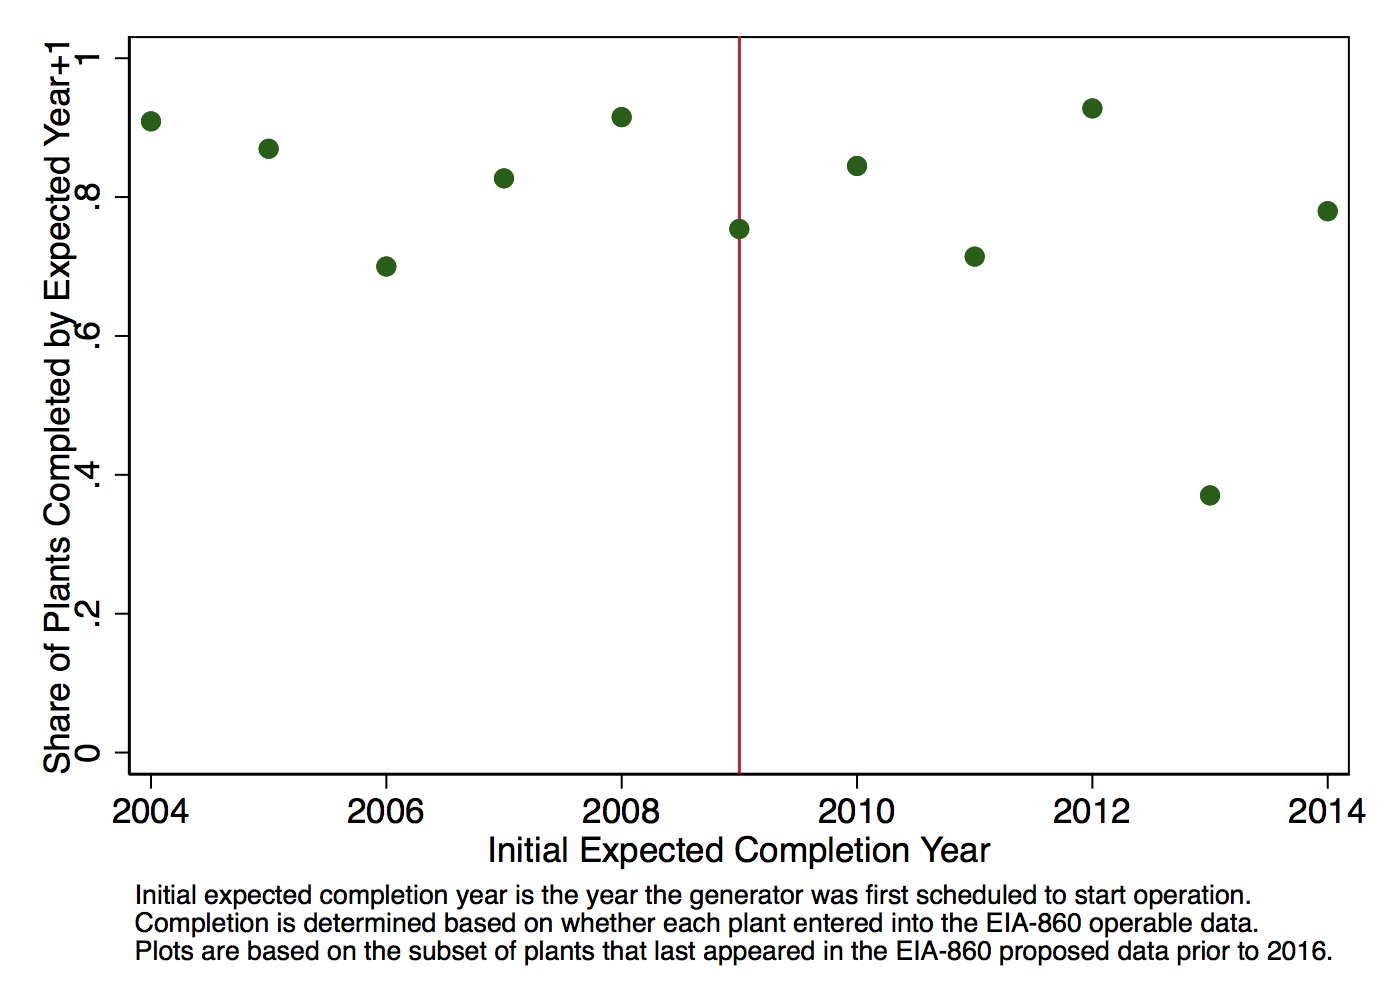
\includegraphics[width=0.75\linewidth]{../output/figures/proposal_data_completed_on_time.png}
\end{figure}


\section{Results \label{sec:results}}

\subsection{Instrumental Variables Strategy\label{sec:results:rd}}

Table~\ref{tab:rdd_cf} reports the instrumental variable results. The sample is restricted to a balanced panel of monthly generation from 2010 to 2014 at wind farms that came online in 2008 or 2009. The dependent variable in each regression is the capacity factor in percentage points.

\begin{table}[h]
\caption{Instrumental Variables Estimates \label{tab:rdd_cf}}
\begin{center} {\footnotesize{}{
\def\sym#1{\ifmmode^{#1}\else\(^{#1}\)\fi}
\begin{tabular}{l*{6}{c}}
\toprule
                &\multicolumn{1}{c}{(1)}         &\multicolumn{1}{c}{(2)}         &\multicolumn{1}{c}{(3)}         &\multicolumn{1}{c}{(4)}         &\multicolumn{1}{c}{(5)}         &\multicolumn{1}{c}{(6)}         \\
\midrule
1603 Grant      &   -5.148\sym{***}&   -3.626\sym{***}&   -2.842\sym{***}&   -3.697\sym{***}&   -2.893\sym{**} &   -3.156\sym{***}\\
                &  (0.915)         &  (0.899)         &  (0.829)         &  (1.351)         &  (1.238)         &  (1.170)         \\
\addlinespace
Regulated       &                  &   -1.562         &   -5.439\sym{***}&                  &   -1.371         &   -5.446\sym{***}\\
                &                  &  (1.712)         &  (1.979)         &                  &  (1.685)         &  (1.970)         \\
\addlinespace
PPA             &                  &   -0.648         &   -2.608\sym{***}&                  &   -0.600         &   -2.618\sym{***}\\
                &                  &  (1.048)         &  (0.927)         &                  &  (1.056)         &  (0.925)         \\
\addlinespace
IPP             &                  &   -1.350         &   -2.554\sym{*}  &                  &   -1.408         &   -2.514\sym{*}  \\
                &                  &  (1.333)         &  (1.351)         &                  &  (1.305)         &  (1.307)         \\
\addlinespace
Potential Capacity Factor&                  &    0.501\sym{***}&    0.551\sym{***}&                  &    0.503\sym{***}&    0.553\sym{***}\\
                &                  & (0.0366)         & (0.0391)         &                  & (0.0368)         & (0.0386)         \\
\addlinespace
Var(Wind Speed) &                  &   0.0400         &   -0.426\sym{***}&                  &   0.0637         &   -0.432\sym{***}\\
                &                  &  (0.148)         &  (0.103)         &                  &  (0.155)         &  (0.107)         \\
\addlinespace
log(Capacity)   &                  &   -0.567         &    0.571         &                  &   -0.605         &    0.580         \\
                &                  &  (0.429)         &  (0.471)         &                  &  (0.430)         &  (0.470)         \\
\midrule
Regression Type &      OLS         &      OLS         &      OLS         &     2SLS         &     2SLS         &     2SLS         \\
Controls        &        N         &        Y         &        Y         &        N         &        Y         &        Y         \\
State FE        &        N         &        N         &        Y         &        N         &        N         &        Y         \\
R-sq.           &    0.372         &    0.557         &    0.660         &        -         &        -         &        -         \\
N               &     8752         &     8752         &     8752         &     8752         &     8752         &     8752         \\
First-stage F-stat.&                  &                  &                  &      148         &      169         &      113         \\
\bottomrule
\end{tabular}
}
} \end{center}
\footnotesize
The dependent variable is the capacity factor in percentage points. Data include a balanced panel of monthly observations from 2010 to 2014 for all wind farms. All models contain year-month dummies. Standard errors clustered by wind farm reported in parentheses.
\end{table}

The primary coefficient of interest ($\delta$) appears in the first row of the table, labeled 1603 Grant. The first three columns present OLS estimates of equation~\ref{eq:second_stage}. Column 1 includes only time (month-year) dummies. The interpretation is that plants receiving output subsidies operated at 5 percentage points lower capacity factor compared to PTC recipients coming online between 2008 and 2009. Column 2 adds controls for plant size and monthly wind quality, as well as dummies for whether the plant is regulated, whether it is owned by an independent power producer, and presence of a power purchase agreement.\footnote{Unless otherwise noted, the same controls appear in every model throughout the paper. Additional discussion of the potential capacity factor and wind speed variables is provided in Appendix~\ref{Appendix:Potential-capacity-factor}.} Consistent with the descriptive evidence above, 1603 and PTC plants differ on observable dimensions, and controlling for these differences reduces the estimated productivity gap. Column 3 adds state fixed effects to account for other unobserved differences in markets and renewable policies across states, which attenuates the relationship further.

Columns 4-6 present IV estimates using the same covariates, instrumenting for 1603 receipt with an indicator for whether the wind farm was eligible for the 1603 program. Conditioning only on month of sample, 1603 plants are 3.7 percentage points less productive than their PTC counterparts. This difference is considerably smaller than the OLS estimate in column 1. Adding controls results in a modestly lower estimated 1603 effect of 2.9 percentage points, and is our preferred specification. Column 6 adds state fixed effects, which effectively discards 25 percent of the sample for which there is no within-state subsidy variation. The estimate splits the difference between the previous two, leaving a 3.2 percentage point gap in productivity across plants choosing the two subsidy types. Our preferred estimate of 2.89implies that 1603 grant recipients would have produced roughly 10percent more power had they claimed the PTC.\footnote{This 10 percent reduction is computed by dividing the estimated 2.89percentage point reduction in capacity factor by the average capacity factor for all 1603 grant recipients of 30.32percentage points.} To provide context for the magnitude of this estimate, note that it is in line with industry claims for how post-construction wind farm optimization services could increase output (see discussion in Section~\ref{sec: Background}). The marginal incentive of the PTC is quite substantial during this time period, providing more than a 40 percent premium over the average price of power sold by wind farms to the grid. As such, the estimate in column 5 implies a supply elasticity of around 0.25. 

\subsubsection*{Robustness Analysis}

We assess the sensitivity of our results to the assumed sample bandwidth. The primary motivation for doing this is concern about violations of the exclusion restricton. Since our instrument is based on time, we are concerned that it will pick up other factors that impact wind farm productivity independent of the policy. Furthermore, although we believe it is highly unlikely that wind farm developers could have made significant changes to projects that began operations in 2009 after first learning about the policy, that possibility becomes more remove as we shorten the sample around the policy introduction. Of course, smaller bandwidths generate smaller samples, lessening the statistical precision of our estimates. Figure~\ref{fig:CFbandwidths} presents coefficients from the preferred specification in column 5 in graphical form using alternative bandwidths ranging from three months to 24 months on each side of the policy change. Although the confidence intervals are large for the very small bandwidths, the results are consistent and reinforce our baseline findings: all specifications suggest receipt of the 1603 grant (investment subsidy) leads firms to produce less electricity than they would have if they had received the PTC (output subsidy). Moreover, the fact that the point estimates remain remarkably stable between nine and twenty-four months assuages concerns that the results are driven mainly by time trends.

\begin{figure}[H]
\caption{IV Estimates using Alternative Bandwidths \label{fig:CFbandwidths}}
\centering{}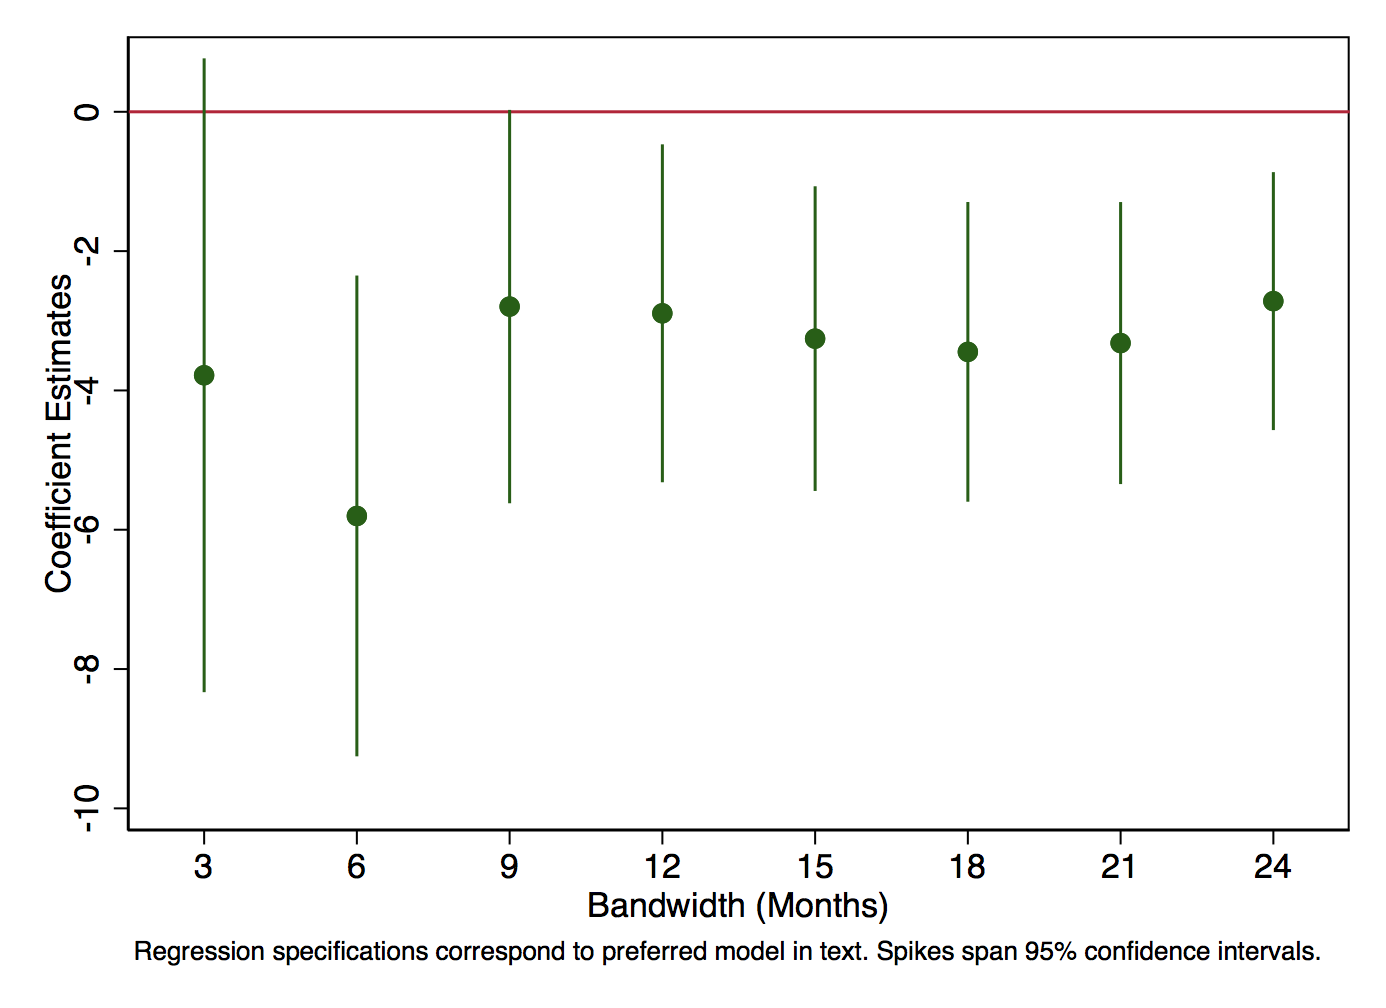
\includegraphics[width=0.75\textwidth]{../output/figures/fuzzyRDD_capfactor_bandwidths_nostateFEs.png}
\end{figure}

We also consider the possibility of trends within the 2008-2009 time period in technology, site quality, and other factors that could have persistent effects on output. Table~\ref{tab:rdd_cf_linear} presents results from a parametric fuzzy regression discontinuity model that includes piecewise linear trends. Unfortunately, given the small sample size, these results are quite noisy. In models 4 and 5, the point estimates are larger in magnitude than the IV estimates, while in model 6 the results are smaller and not statistically distinguishable from either the IV estimates or zero. The variability in these estimates may be the result of weak instruments, as they have relatively small first-stage F-statistics.

\subsection{Matching Strategy}

We now present results from the matching estimator described in Section~\ref{subsec:Matching}. We match exactly on several categorical variables (geography, wind quality class, regulatory status, and entity type) and two coarsened continuous variables (capacity and design wind speed).\footnote{In this analysis, we match on two wind quality measures collected by the EIA, design wind speed and wind class. An alternative would be to match on the realized potential capacity factor, which we construct and use as a control at the month level, averaged over the sample. We prefer the EIA measures because they are directly reported to the EIA, and likely more accurate in the cross section. These two measures are also widely used in the industry, with wind class (a categorization of site wind variability) used as a critical determinant of which turbines can safely be placed at a location. Moreover, the conceptual exercise here is to match similar \textit{sites} in the pre and post policy period, while the potential capacity factor combines both site and time-varying technology changes. With that said, the results are qualitatively similar when we match on potential capacity factor instead. These are presented in appendix Tables~\ref{tab:matching_group_ptnlcf} and \ref{tab:matching_table_cf_ptnlcf}.} This procedure selects all pre-period wind farms within the same coarsened cell in the covariate space as each post-period wind farm.

Table~\ref{tab:matching_balance} compares pre- and post-period entrants after using coarsened exact matching with state as the geography. Of the 465 wind farms in our sample entering between 2005 and 2012, 204 lie within the common support of these variables across the two policy periods.\footnote{The number of post-period matches is higher than pre-period matches because more post-period plants fall within the same coarsened cell than do pre-period plants.} The number of post-period 1603 matches is about double the number of PTC matches, which is in line with their underlying population probabilities. T-tests confirm that this restricted sample is in fact balanced across the two time periods on the matched dimensions. In particular, the two dimensions that were imbalanced in the IV sample, capacity and IPP status, are now statistically equivalent across the pre and post periods in this sample by construction. 

\begin{table}[h]
\caption{Matching Balance \label{tab:matching_balance}}
\begin{center}
\begin{tabular}{lcccc}
\hline \noalign{\smallskip} & Pre & Post & Difference & p-value\\
\noalign{\smallskip}\hline Nameplate Capacity (MW) & 101.91 & 105.39 & 3.48 & 0.74\\
Turbine Size (MW) & 1.78 & 1.89 & 0.11 & 0.05\\
Design Wind Speed (MPH) & 17.92 & 17.46 & -0.45 & 0.14\\
Regulated & 0.09 & 0.09 & 0.00 & 1.00\\
IPP & 0.89 & 0.89 & 0.00 & 1.00\\
PPA & 0.82 & 0.77 & -0.05 & 0.42\\
Potential Capacity Factor & 36.76 & 37.39 & 0.63 & 0.53\\
Capacity Factor & 34.01 & 32.80 & -1.21 & 0.14\\
\hline \noalign{\smallskip}Wind Farms & 86 & 118 &  & \\
1603 Recipients &  & 83 &  & \\
\noalign{\smallskip}\hline\end{tabular}\\
\end{center}

\footnotesize

Each row contains a two-sample t-test for a difference in means between wind farms that came online before versus after January 1, 2009 that meet sample restrictions described in Section~\ref{sec:Data} and are selected using coarsened exact matching. See text for more details on the matching procedure. Regulated and IPP are identical across samples by construction. Regulated, IPP, and PPA are binary variables. Potential Capacity Factor and Capacity Factor are ratios (scaled by 100).
\end{table}

Table~\ref{tab:matching_group} reports the results from regressions estimated through variations of this matching strategy with a balanced sample of monthly wind farm production data. As before, the dependent variable in each regression is the capacity factor measured in percentage points. All models include the same controls as our preferred IV regressions as well as dummies for cohort (i.e., the first year each wind farm generated electricity). Column 1 presents estimates from estimating OLS on the full sample including all 465 wind farms entering during the pre- or post-period. Column 2 restricts the sample to plants matched across periods. Column 3 includes matched group fixed effects. Column 4 interacts those group fixed effects with year of sample, allowing for unobserved factors that affect specific groups and vary over time. Column 5 includes group-year-month fixed effects. 

Simply restricting the sample to observably similar plants across periods increases the estimated impact of the 1603 grant from 2.9 to 4 percentage points. This suggests that there are low productivity PTC plants and/or high productivity 1603 plants that do not lie in the common support across periods. Allowing for increasingly time-varying group level unobservables has remarkably little effect on the estimates. The estimated productivity reduction in column 4 of 3.72percentage points (12percent) is similar to our preferred IV estimate, despite relying on different identifying assumptions.

\begin{table}[h]
\begin{centering}
\caption{Matching Estimates \label{tab:matching_group}}
{
\def\sym#1{\ifmmode^{#1}\else\(^{#1}\)\fi}
\begin{tabular}{l*{5}{c}}
\toprule
                    &\multicolumn{1}{c}{(1)}         &\multicolumn{1}{c}{(2)}         &\multicolumn{1}{c}{(3)}         &\multicolumn{1}{c}{(4)}         &\multicolumn{1}{c}{(5)}         \\
\midrule
1603 Grant          &      -2.942\sym{***}&      -3.975\sym{***}&      -3.862\sym{***}&      -3.716\sym{***}&      -3.633\sym{***}\\
                    &     (0.719)         &     (1.063)         &     (1.019)         &     (1.033)         &     (1.159)         \\
\midrule
Sample              &         All         &     Matched         &     Matched         &     Matched         &     Matched         \\
FEs                 &       State         &       State         &       Group         &     Group*Y         &   Group*Y*M         \\
R-sq.               &       0.615         &       0.623         &       0.632         &       0.642         &       0.762         \\
N                   &       21303         &       10106         &       10106         &       10106         &       10106         \\
\bottomrule
\end{tabular}
}

\par\end{centering}
\footnotesize

The matched sample was constructed using coarsened exact matching on state, wind quality class, regulatory status, entity type, capacity, and design wind speed. All models include the controls listed in the IV models in Table~\ref{tab:rdd_cf}: log capacity, potential capacity factor, and wind speed variance, as well as dummies for whether the plant is regulated, whether it is an IPP, the presence of a PPA, and month of sample. All models also include cohort dummies. Standard errors, clustered at the plant level, are reported in parentheses.
\end{table}

\subsubsection*{Robustness Analysis}

The most restrictive matching criteria in the previous exercise is the requirement that pre and post plants be in the same state. In order to explore the impact of this assumption, and to incorporate more plants into the analysis, we re-estimate the model from column 4 under different geographic restrictions (Table~\ref{tab:matching_table_cf}). As above, all models use coarsened exact matching on geography, wind quality class, regulatory status, entity type, capacity, and design wind speed. In addition, column 1 matches on NERC region as well as an indicator for whether the plant is in an ISO. Column 2 matches on the specific ISO a plant participates in, and column 3 matches on both NERC region and ISO. Finally, column 4 matches on state, repeating column 4 from the previous table. In addition to controls, month of sample dummies, and matched group-year dummies, each of the first three models also include state fixed effects to account for differences in state-level renewable policies. As in the previous table, the results increase slightly as increasing restrictions are placed on the matching procedure. However, we cannot statistically discern among the coefficient estimates.

\begin{table}[h]
\begin{centering}
\caption{Sensitivity of Matching Estimates to Geographic Restrictions \label{tab:matching_table_cf}}
{
\def\sym#1{\ifmmode^{#1}\else\(^{#1}\)\fi}
\begin{tabular}{l*{4}{c}}
\toprule
                    &\multicolumn{1}{c}{(1)}         &\multicolumn{1}{c}{(2)}         &\multicolumn{1}{c}{(3)}         &\multicolumn{1}{c}{(4)}         \\
\midrule
1603 Grant          &      -2.989\sym{***}&      -3.362\sym{***}&      -3.472\sym{***}&      -3.716\sym{***}\\
                    &     (0.918)         &     (0.961)         &     (1.032)         &     (1.033)         \\
\midrule
\# Pre-PTC          &         108         &         100         &          90         &          86         \\
\# Post-PTC         &          54         &          51         &          44         &          35         \\
\# Post-1603        &         116         &          87         &          78         &          83         \\
Region              & Nerc-1(ISO)         &         ISO         &    Nerc*ISO         &       State         \\
R-sq.               &       0.634         &       0.677         &       0.661         &       0.642         \\
N                   &       13439         &       11724         &       10577         &       10106         \\
\bottomrule
\end{tabular}
}

\par\end{centering}
\footnotesize

Matched samples constructed using coarsened exact matching on geographies listed in the table, wind quality class, regulatory status, entity type, capacity, and design wind speed. All models include the controls listed in the IV models in Table~\ref{tab:rdd_cf}: log capacity, potential capacity factor, and wind speed variance, as well as dummies for whether the plant is regulated, whether it is an IPP, the presence of a PPA, and month of sample. All models also include cohort dummies, matched group-year fixed effects, and state fixed effects. Standard errors, clustered at the plant level, are reported in parentheses.
\end{table}

\subsection{Section 1603 Program Evaluation\label{sec:results:eval}}

The previous sections provided evidence that 1603 recipients would have generated significantly more output had they claimed the PTC. In order to calculate the full effect of the 1603 program, however, we need to consider that some 1603 recipients may not have found it profitable to enter without investment subsidies. Section \ref{subsec:EntrySelection}  presented graphs which showed no discernable shift in entry rates during the 1603 period. In this section, we perform a back-of-the-envelope calculation to identify ``marginal'' plants, i.e., power plants claiming the 1603 grant that appear profitable under the investment subsidy but not the PTC. We describe this calculation briefly here and provide additional details in Appendix~\ref{Appendix:Profitability-calculation-detail}.

We specify the following discounted profit functions under each subsidy regime:
\begin{align*}
\pi_i^{1603}&=\sum_{t=1}^{t=25}\left(\frac{1}{1+r}\right)^{t}(p_{it}-c_{t})Q_{it}^{1603}-(0.7)F_i \\
\pi_i^{PTC}&=\sum_{t=1}^{t=25}\left(\frac{1}{1+r}\right)^{t}(p_{it}-c_{t})Q_{it}^{PTC}+\sum_{t=1}^{t=10}\left(\frac{1}{1+r^{PTC}}\right)^{t}(PTC)Q_{it}^{PTC}-F_i
\end{align*}
Wind farms are assumed to remain in service for 25 years ($t$), with output predicted to decay at a linear rate estimated using the full panel of wind farms. Plant-specific output prices ($p_{it}$) are computed based on revenue and sales quantities reported on EIA Form 923.\footnote{Of the 192 1603 plants in the sample, six do not report any resale quantities in the EIA data and are thus excluded from this analysis. Future prices are assumed to remain constant in real terms.} We also include in $p_{it}$ estimated marginal revenue from the sale of RECs under state-level renewable portfolio standards using data from Marex Spectron and Lawrence Berkeley National Laboratory. Operations and maintenance costs ($c_{t}$) of \$9/MWh are taken from \citet{wiser_2015_2016}. Marginal net revenue is combined with an estimate of output ($Q_{it}$) to construct annual net revenue, which is discounted at an assumed 5 percent real interest rate ($r$). Fixed investment costs ($F_i$) are obtained by dividing the observed 1603 grant award amount from Treasury by the fraction of investment costs covered by the program (0.3).\footnote{Wind farms are also eligible for accelerated depreciation, which we assume is equal to 10 percent of investment costs. In a 2010 White House Memorandum to the President, leaked to multiple news outlets, the Shepherds Flat Wind Farm in Oregon was revealed to have approximately \$200 million in accelerated depreciation benefits on a \$2.1 billion investment. \citet{borenstein_private_2015} also finds accelerated depreciation benefits on the order of 10-12 percent of investment costs for solar power. } 

Output under the 1603 ($Q_{it}^{1603}$) is obtained by converting predicted capacity factor ($q_{it}^{1603}$) to electricity generation using plant capacity. Counterfactual output under the PTC ($Q_{it}^{PTC}$) is obtained by increasing $q_{it}^{1603}$ by 3.3 percentage points (reflecting the average of our preferred IV and matching results) for the first ten years of operation, and then converting this to electricity generation using plant capacity. During this period, each MWh produced also generates \$23 in tax credits, in addition to the marginal revenue collected under the 1603. However, these tax credits need to monetized, and are thus less valuable than cash. As discussed in Section~\ref{sec: Background}, the creation of the 1603 grant program reflected concerns that wind developers could not find tax equity partners\textemdash large financial companies with sufficient tax liabilities to monetize the PTC\textemdash due to the financial crisis. \citet{bolinger_analysis_2014} reports that the tax equity yield remained fairly stable at six percent over 2005-2007. Over 2008-2009, this yield increased by as much as 450 basis points, reflecting the contraction in tax equity supply. In order to account for this additional cost of monetizing tax equity, we discount the PTC revenue streams by an assumed 8 percent tax equity yield, which is the modal value of the tax equity yield over 2009-2012 presented in \citet{bolinger_analysis_2014}.\footnote{Using the maximum observed yield of 10.5 percent does not meaningfully change the results. An alternative approach would be to use the same discount rate for all revenue streams but deflate nominal PTC revenues to reflect their real value to the wind farm. We do this using a prior estimate that firms value each PTC dollar at \$0.85 \citep{johnston_non-refundable_2019} and find that it does not meaningfully change our results.}

Table~\ref{tab:policyeval} summarizes these two constructed profit measures for 1603 grant recipients. The first two columns of the table report predicted lifetime output along with the total observed 1603 award amount. The third column presents the ratio of total subsidy to total \textit{discounted} output, which can be interpreted as the public funds levelized cost of energy (LCOE). The final three columns present predicted output, subsidy in present value terms, and public funds LCOE for these projects had they claimed the PTC instead of the 1603 grant. Plants are assigned to one of three groups: an always profitable group ($\pi^{1603}>0$ \& $\pi^{PTC}>0$), a marginal group ($\pi^{1603}>0$ \& $\pi^{PTC}<0$), and a never profitable group ($\pi^{1603}<0$ \& $\pi^{PTC}<0$).\footnote{There are two1603 recipients that we find to be profitable under the PTC but not under the 1603. These discrepancies could be due to data limitations (e.g., inaccurate prices) or a result of investments that turned out to be unprofitable \textit{ex post}. We include them in the always profitable group for this analysis, as the fact that we underestimate their expected profits under the 1603 program gives us no reason to believe we overestimate their expected profits under the PTC.} Somewhat surprisingly, 25percent of 1603 recipients fall into this final category. There are many potential reasons for this. One simple explanation is mean reversion. For some facilities, only a handful of years are observed to construct output projections, so our approach could understate the profits of wind farms that had low output realizations during the years we observe. We may have also underestimated state and local subsidies or overestimated O\&M costs and discount rates for some facilities. However, even if we had perfectly accounted for all of these factors, it is likely that some plants that appeared profitable \emph{ex ante} will be unprofitable \emph{ex post} due to low price and wind realizations.

\begin{table}[H]
\caption{Estimated Subsidy by Group\label{tab:policyeval}}

\vspace{-15pt}

\begin{center}
\footnotesize
\newcolumntype{Y}{>{\raggedleft\arraybackslash}X}
\begin{tabularx} {\textwidth} {@{} l Y Y Y Y Y Y Y Y Y Y Y Y Y Y Y Y@{}} \\
\toprule
& & \multicolumn{3}{c}{1603} & \multicolumn{3}{c}{PTC} \\
\cmidrule(l{.75em}){3-5} \cmidrule(l{.75em}){6-8}
Group & N & Output (MMWh) & Subsidy (\textdollar M) & Subsidy (\textdollar/MWh) & Output (MMWh) & Subsidy (\textdollar M) & Subsidy (\textdollar/MWh) \\
\midrule
Always Profitable&132&598&7,120&18.68&634&7,009&17.12 \\
Marginal&7&17&334&30.41&18&215&17.79 \\
Never Profitable&47&186&2,621&21.91&198&2,265&17.47 \\
\bottomrule
\addlinespace[.75ex]
\end{tabularx}
\par
\normalsize
%\scriptsize{\emph{Source: }#}
\end{center}

\footnotesize

Estimated electricity generation and subsidy for 1603 recipients, divided into three groups depending on their estimated profitability under the 1603 grant and the PTC. Output is a lifetime sum without discounting, Subsidy is in net present value terms, and Subsidy per MWh is constructed by taking the ratio of the sum of discounted subsidy expenditures to the sum of discounted electricity generation as in the definition of the LCOE. The first set of numbers correspond to outcomes under the subsidy they chose. The second set presents a counterfactual for the subsidy they did not choose.
\end{table}

Estimating the full effect of the 1603 program requires taking a stand on the counterfactual entry status of the never-profitable group. One possibility is to assume that the never-profitable plants are in fact marginal, and would not have entered without the 1603 grant program. Under this assumption, the 1603 program increased lifetime wind production by 167MMWh (reflecting the difference between the total output under the 1603 column and the output for the always-profitable group under the PTC column). This would also imply that the 1603 grant increased the average public cost per wind MWh from \$17.12to \$19.69\unskip, a 15percent reduction in cost-effectiveness.

In our view, this assumption is unlikely, given the graphical evidence on entry rates presented in Figure~\ref{fig:proposed_completed_on_time}. Instead, it seems more plausible that the apparent lack of profitability of the third group in Table~\ref{tab:policyeval} implies a policy-invariant unobservable (possibly in expectation) that would have encouraged these wind farms to enter with or without the 1603 grant. Under this assumption, the 1603 grant program screened in just 17MMWh of production at the sevenmarginal plants. At the same time, production at inframarginal plants declined. Under this assumption, our preferred assumption, total wind output would have been modestly \emph{higher} without the 1603 program (by 31MMWh, or 4percent), while total government expenditure would have declined by \$801million. The average public cost per wind MWh would have increased from \$17.20to \$19.69\unskip, a 14percent reduction in cost-effectiveness.

Let us acknowledge a few caveats to this analysis. First, our estimate of always-profitable wind farms may be too high based on our assumption of the discount rate associated with the PTC. The tax equity supply shock associated with the financial crisis motivated the creation of the Section 1603 grant program. This decline in supply is evident in the spike in tax equity yields in 2009. We employed a higher rate for discounting the PTC streams in evaluating the counterfactual for our 1603 grant-claiming wind farms to reflect the increase in tax equity yields during this time period. This higher discount rate may be valid for evaluating the marginal project, but it could be too low when considering the counterfactual of all of the 132always-profitable 1603 grant claimants going to the tax equity market to monetize their production tax credits. Second, note that our conclusions about the Section 1603 grant program reflect the specific policy design of a grant equal to 30 percent of eligible investment costs relative to the specific PTC design of awarding \$23 per MWh of output. Modifying either policy parameter could influence the cost-effectiveness of the investment and output subsidy approaches. 

\section{Discussion\label{sec:Discussion}}

\subsection{Mechanism \label{sec:Mechanism}}

Our empirical results are consistent with a model of convex effort costs on the intensive margin. While the true marginal cost of operation is likely zero in any given hour, wind farm operators perform costly maintenance activities over longer time horizons to ensure their turbines operate efficiently. Turbines are large, mechanical devices, periodically placed under extreme stress. From time to time, one component breaks and the turbine needs to shut down as a safety precaution. Operators need to quickly identify (or even better, \textit{predict}) such failures, and send a technician to scale the device and fix the problem. Wind farms that receive a higher price for their output have a larger opportunity cost of foregone production, and thus a greater incentive to prevent and minimize the downtime associate with turbine failures. 

On a more continual basis, poor management can cause operable turbines to produce well below their maximum potential. In response to this, a robust turbine service consulting market has developed, with providers purporting to optimize operations and boost output. For example, General Electric offers a product called ``PowerUp'', which it describes as ``a customized suite of software and hardware-enabled technologies created to increase a wind farm's output by up to 10\%, taking into account environmental conditions.''\footnote{Source: \href{https://www.gerenewableenergy.com/wind-energy/turbine-services/platform-upgrades}{General Electric website} (accessed 1/29/2018). Another example is Uptake, an analytics firm that brings artificial intelligence to industrial devices including wind farms and claims that it can ``Improve your annual energy production, increase turbine days available and make more accurate power forecasts.''} While we do not have any information on the takeup rate of such services across PTC and 1603 plants, the fact that this advertised productivity gain matches our estimated treatment effect suggests that a ten percent increase in production through the channel of better, more intense, plant management is plausible.

Even in the absence of convex operating costs, output subsidies could mechanically encourage more output by incentivizing production when the marginal willingness to pay for electricity is below zero. In electricity markets, prices sometimes fall below zero during periods of low demand due to a combination of inflexible supply, prohibitively expensive storage, and transmission constraints. In these periods, wind farm operators who receive the PTC should be willing to pay at least as much as the value of the subsidy to be dispatched each time period, whereas 1603 recipients would have less of an incentive to supply electricity.\footnote{Both types of firms may receive other subsidies or be party to contracts that give them an incentive to produce electricity when the price is negative. We focus here on the differential incentives attributable to the Federal subsidies we study.}

How much of the difference in output across PTC and 1603 plants can be attributed to negative prices? If we observed hourly bids and clearing prices for all the plants in our sample, we could compute this number directly. Unfortunately, these data are not available. In lieu of this, we first collect high-frequency wholesale electricity prices at all nodes (i.e., locations) for six large U.S. electricity markets. For each wind farm in our sample, we use these data to compute the frequency of negative prices at the closest node on a monthly basis from 2011 to 2014. Appendix~\ref{Appendix:NegativePrices} provides more detail on these price data and presents summary statistics. Negative price shares vary considerably across time and space, however averages in excess of our estimated 1603 capacity factor decline are not uncommon (Appendix Table \ref{tab:Frequency-of-Negative}). 

Comparing these averages to our estimated 1603 productivity effect requires making an assumption about the correlation between negative price events and the availability of each wind farm to be dispatched. As was discussed above, on average wind farms only have sufficient wind conditions to operate about one-third of the time. If we assume that availability perfectly coincides with negative prices, then these marginal frequencies can be compared directly to the estimated policy effects. If they are uncorrelated, then these marginal frequencies should be divided by three (on average). We estimate this correlation directly by running the following regression on the full sample of wind farms we are able to match to pricing nodes: 

\begin{equation}
    q_{it}=\alpha \left\{ \mbox{Share}_{it} < 0 \right\} + \beta D_{i} \left\{ \mbox{Share}_{it} < 0 \right\} + \nu_i + \mu_t +\epsilon_{it}\label{eq:frac0} ,
\end{equation}

\noindent where $q_{it}$ is the capacity factor and $\mbox{Share}_{it}$ is the share of hours each month when the price at the nearest node was below zero (both in percentage points). $\nu_i$ and $\mu_t$ are plant and month-of-sample fixed effects, and $D_i$ is an indicator for whether plant $i$ received a 1603 grant, as in equation \ref{eq:second_stage}. We also include potential capacity factor and wind variance as controls. Table \ref{tab:frac0_1603} presents the results. $\beta$ reflects the extent to which negative prices \textit{differentially} affect production by 1603 plants. The estimated effect of a 29 percentage point reduction in capacity factor for every percentage point increase in the share of negative price hours is statistically indistinguishable from the average capacity factor of 1603 plants in the sample, 30, presented in the bottom of the table. We interpret this as evidence that eliminating hours with negative prices would generate the same differential output response as would an equivalent increase in the number of hours in which 1603 plants operate at their observed capacity factor.

\begin{table}[h]
    \caption{Negative Prices and 1603 Plant Productivity \label{tab:frac0_1603}}
    \begin{center} {\footnotesize{}{
\def\sym#1{\ifmmode^{#1}\else\(^{#1}\)\fi}
\begin{tabular}{l*{1}{c}}
\toprule
                &\multicolumn{1}{c}{Capacity Factor}\\
\midrule
Share $<$ 0     &    0.057\sym{*}  \\
                &  (0.023)         \\
\addlinespace
Share $<$ 0 - 1603 Grant&    -0.29\sym{***}\\
                &  (0.064)         \\
\midrule
Mean(Y) - 1603 Grant&    30.12         \\
R-sq.           &     0.70         \\
N               &    13638         \\
\bottomrule
\end{tabular}
}
} \end{center}
    \footnotesize
    
    Results from ordinary least squares estimation of equation~\ref{eq:frac0}. The dependent variable, capacity factor, and the share of negative prices are both in percentage points. The model includes potential capacity factor, wind speed variance, and plant and month-of-sample fixed effects. Data include a balanced panel of monthly observations from 2011 to 2014 for all wind farms. Standard errors clustered by wind farm reported in parentheses.
\end{table}

To approximate the contribution of negative prices to the estimated 1603 treatment effect, we re-estimate our preferred IV and matching regressions after adjusting the dependent variable for negative prices on the basis of this evidence. Specifically, for 1603 plants, we compute the product of the observed capacity factor and the share of negative prices at the nearest node, and add this number to the dependent variable (capacity factor). The results are presented in Table~\ref{tab:regs_negative_prices}. These results suggest that negative prices explain roughly 40 percent, at most, of the electricity generation increase caused by replacing investment subsidies with output subsidies.\footnote{Sometimes wind farms are not dispatched even when they bid below the market clearing price. Disaggregated high-frequency data on such ``curtailment'' is not available, so it is difficult to know how common this is during periods when prices are positive, and would thus not be captured in this analysis. According to \cite{bird_wind_2014}, units are typically selected for curtailment based on characteristics that are unrelated to subsidy status (e.g., local transmission congestion). However, the exhaustive review of curtailment policies in \cite{bird_wind_2014} did mention one utility, PSCO, which curtailed PTC plants second, all else equal, to avoid paying their PTC compensation. Given the levels of curtailment described in the report and our understanding that this example is an exception rather than the rule, we believe differential curtailment is unlikely to explain a large portion of our estimated effect.} 

\begin{table}[h]
    \caption{Effect of Negative Prices on Preferred Estimates \label{tab:regs_negative_prices}}
    \begin{center} {\footnotesize{}{
\def\sym#1{\ifmmode^{#1}\else\(^{#1}\)\fi}
\begin{tabular}{l*{4}{c}}
\toprule
                    &\multicolumn{1}{c}{(1)}         &\multicolumn{1}{c}{(2)}         &\multicolumn{1}{c}{(3)}         &\multicolumn{1}{c}{(4)}         \\
\midrule
1603 Grant          &      -2.893\sym{**} &      -2.542         &      -3.716\sym{***}&      -2.184\sym{**} \\
                    &     (1.238)         &     (1.769)         &     (1.033)         &     (1.099)         \\
\midrule
Estimator           &          IV         &          IV         &       Match         &       Match         \\
Negative Price Adjustment&          No         &         Yes         &          No         &         Yes         \\
N                   &        8752         &        6336         &       10106         &        7054         \\
\bottomrule
\end{tabular}
}
} \end{center}
    \footnotesize
    
    Results from our preferred IV and matching estimators with and without adjusting for the frequency of negative prices. Data include a balanced panel of monthly observations from 2011 to 2014 for all wind farms. Standard errors clustered by wind farm reported in parentheses.
\end{table}

While it is useful to understand the mechanism behind our productivity estimates, the extent to which they are driven by negative prices does not necessarily alter their policy implication. The motivation for subsidizing wind energy is to displace conventional, polluting generation with zero-emissions electricity. This logic does not necessarily change simply because the equilibrium wholesale price is below zero, as the full social value of wind energy depends on the emissions intensity of marginal generation during these hours. In other words, the wholesale electricity price is not a sufficient statistic for the welfare impact of a given unit of electricity generated from wind. 

Determining whether the marginal emissions displaced from wind energy are higher or lower during periods of negative prices is beyond the scope of this paper. However, \citet{callaway_location_2018} provide estimates of the average marginal operating emissions rates of generating resources by hour of day and season for each ISO. We use their data to provide evidence on both the level of emissions rates and the correlation between negative prices and emissions rates. Detailed results are again presented in Appendix~\ref{Appendix:NegativePrices}. In all six electricity markets, average marginal operating emissions rates are positive and large during all hours and seasons. In four of the six electricity markets, average marginal emissions are actually \emph{higher} during seasons and hours of the day where negative prices are more common. Thus, in these markets, the fact that some of the estimated treatment effect comes from willingness to operate at negative prices could be considered a feature of subsidizing output rather than subsidizing investment, not a bug. The purpose is to reduce emissions, and the net benefits from emissions reductions can still be positive, even when prices are not.

With that being said, the fact that there is substantial variation in average marginal operating emissions rates, but no variation in the subsidy awarded for each unit of electricity under the PTC, indicates that the PTC is a poor substitute for a Pigouvian emissions tax. In the two markets where emissions are negatively correlated with negative prices, California and New England, nuclear power and hydropower often provide zero-emissions baseload generation. In these regions, output subsidies to renewable generators could actually \emph{undermine} long-run, system-wide emissions objectives. By reducing revenue for these high capacity factor, high fixed cost, low-emissions electricity sources, the PTC could expedite their retirement. It is unlikely that this effect dominates the environmental benefits of the PTC, but this highlights another shortcoming of subsidizing renewable electricity relative to pricing the emissions externality directly.

\subsection{Input Mix Distortions}

The 1603 grant program was a non-uniform input subsidy. Certain capital inputs, most notably wind turbines, were subsidized, while other inputs, like land and transmission equipment, were not. When faced with a shift in the relative price of inputs, firms will likely alter their input mix, either by employing relatively more subsidized inputs or by selecting higher quality subsidized inputs \citep[as found for other industries in][]{goolsbee_taxes_2004}. Whether this input response increases or decreases public cost-effectiveness depends on the substitutability of inputs and the elasticity of output with respect to inputs at the margin \citep{parish_relative_1982}. However, such distortions are clearly socially inefficient. 

Our previous analysis estimated the productivity effect of removing output subsidies \textit{conditional on the input mix} of each firm.\footnote{Specifically, our preferred specifications for both estimation strategies include plant-turbine-specific estimates of potential output each month.} This was partially motivated by the fact that, due to long lead times, plant inputs were fixed during the early part of the 1603 program. However, the program did run for four years, likely giving some later developers time to tailor their investments to the 1603 grant. In this section, we look for evidence of a shift in the input mix for plants selecting the 1603 grant program relative to the input mix for plants selecting the PTC as inputs became more flexible over time. 

The effect of the policy change on the total capacity of any project is ambiguous, given that the output subsidy also encourages larger projects through increased operating revenue. However, the fact that turbines are subsidized while land is not suggests that, conditional on project size, 1603 developers should prefer to use larger turbines and less land. Figure \ref{fig:input_trends} plots the average turbine size (megawatts, top panel) and footprint (square miles per turbine, bottom panel) by year of entry and subsidy type. In general, turbines have been getting larger over time. While there is no difference in these raw averages across subsidy types in the first two years of the 1603 program, towards the end of the sample, plants selecting the capital subsidy use substantially larger turbines.  Conversely, 1603 plants were using relatively more land when inputs were likely fixed, and substantially less during the latter half of the program when there may have been time to adjust. 

\begin{figure}[H] \centering
    \caption{Input Choices by Year of Entry and Subsidy Type \label{fig:input_trends}}
    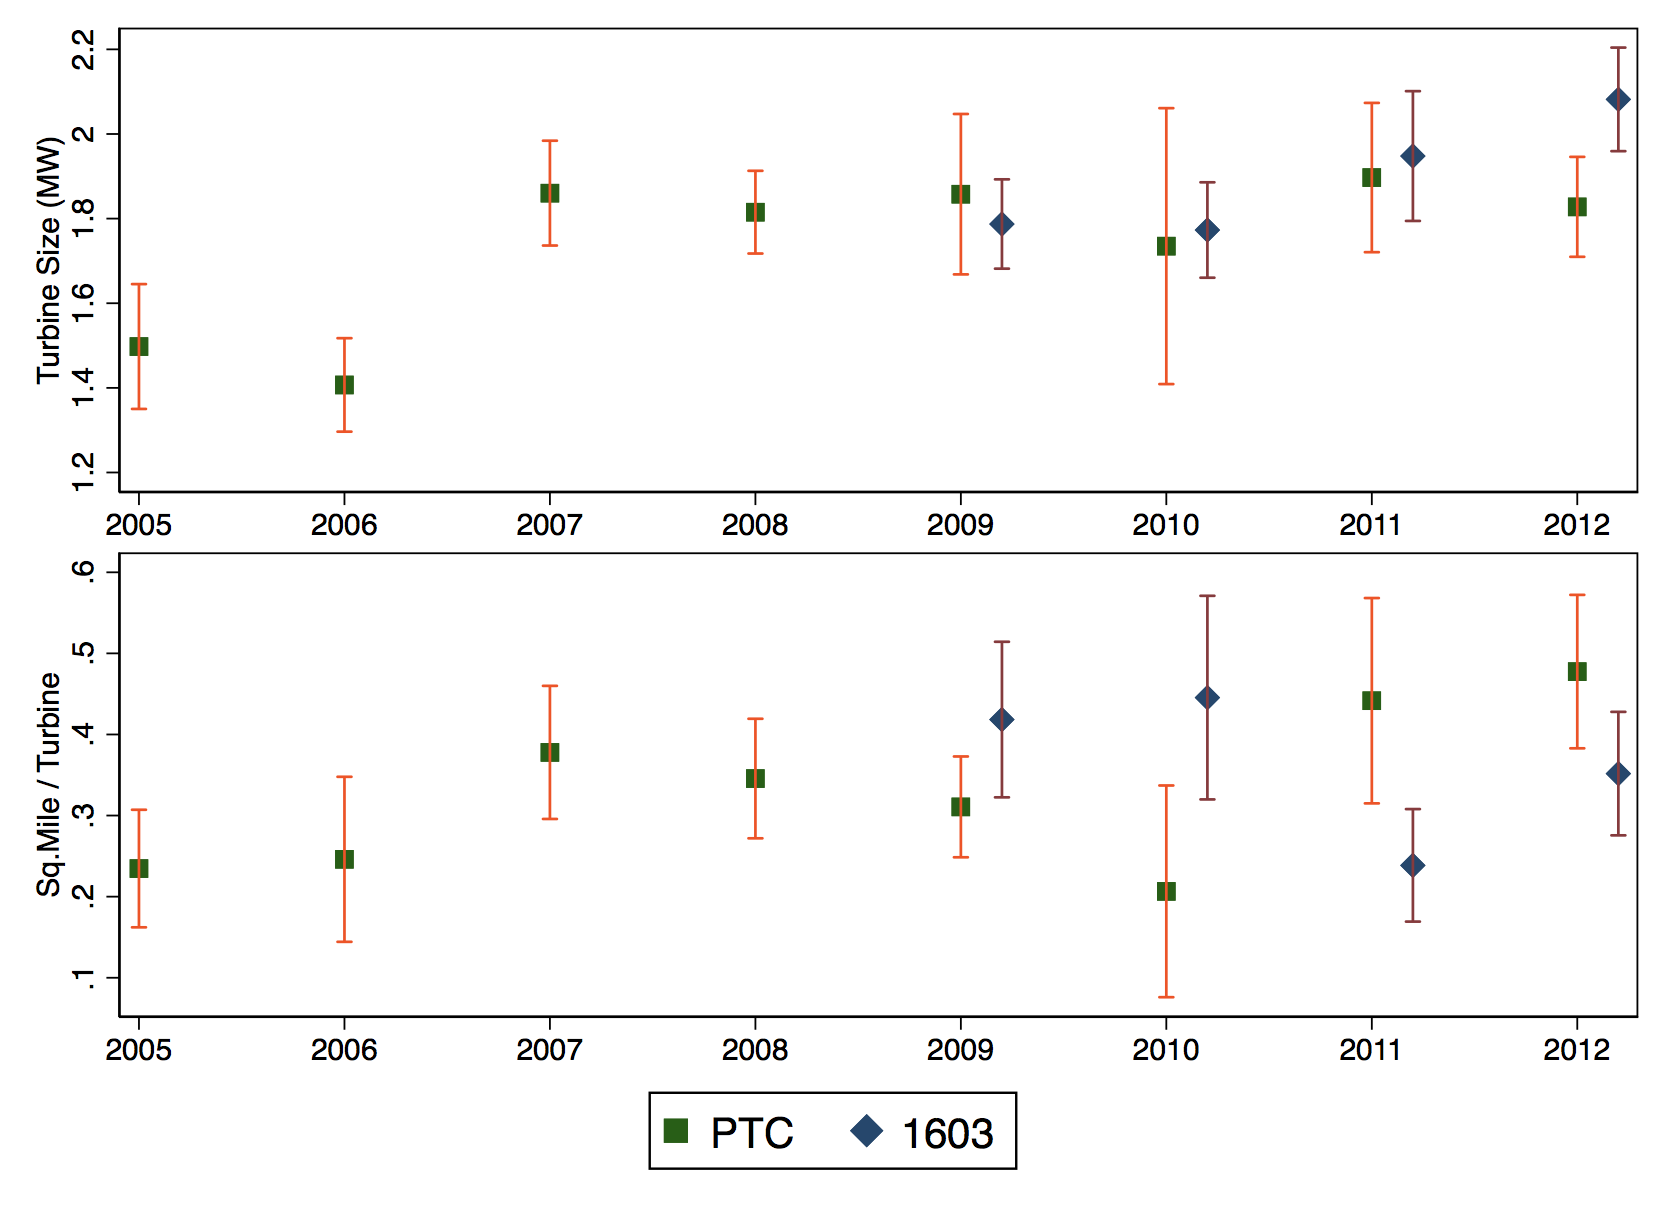
\includegraphics[width=0.85\linewidth]{../output/figures/input_trends.png}
\end{figure}

Given the small sample, these apparent differences in input choices could be driven by other changes in project composition over time. We test for time-varying differences in the groups using the following regression, 

\begin{equation}
y_{i}= \alpha\text{\{1603\}} + \sum_{t=2010}^{t=2012} \alpha^t\text{\{1603 \& $year_i =t$ \}} + \beta X_i + \eta_{year} + \epsilon_{i},\label{eq:capitalbias}
\end{equation}
where 1603 indicates that a wind farm claimed the 1603 grant, $year_i$ is the year that a plant entered, and $\eta_{year}$ represents year of entry fixed effects to account for trends in these variables over time that are common across subsidy groups. In some specifications we include additional characteristics in $X_i$. As specified, $\alpha$ reflects pure selection, based on the difference in inputs between projects that select the 1603 and PTC during 2009 when land and turbine choices were fixed. The remaining $\alpha^t$ then reflect how this selection changed over time. 

Table~\ref{tab:input_mix_regs} reports the results. In column 1, the dependent variable is turbine size, and we omit the control vector $X_i$. Consistent with the picture in the top panel of figure \ref{fig:input_trends}, 1603 plants start off with indistinguishable turbines in 2009, but then become significantly larger at the end of the sample. Column 2 adds controls for project size, regulatory and IPP status, and wind speed, and column 3 adds state fixed effects as well. The estimated change in the relative size of PTC and 1603 plants is large and significant in all three specifications, and represents a roughly 15 percent increase in relative turbine size as developers adjust their inputs. Columns 4 through 6 repeat these regressions using plant footprint (square miles per turbine) as the dependent variable. In the early years, when sites were selected prior to knowledge of the subsidy, 1603 plants are actually less densely packed than those receiving the output subsidy. But in the latter years, this selection is reversed, representing a more than 50 percent decline in footprint per turbine. 

\begin{table}[H]
\begin{centering}
\caption{Change in Wind Farm Characteristics over Time\label{tab:input_mix_regs}}
\par\end{centering}
\begin{centering}
{\footnotesize{}{
\def\sym#1{\ifmmode^{#1}\else\(^{#1}\)\fi}
\begin{tabular}{l*{6}{c}}
\toprule
                &\multicolumn{1}{c}{(1)}         &\multicolumn{1}{c}{(2)}         &\multicolumn{1}{c}{(3)}         &\multicolumn{1}{c}{(4)}         &\multicolumn{1}{c}{(5)}         &\multicolumn{1}{c}{(6)}         \\
\midrule
1603 Grant      &   -0.070         &   -0.055         &   -0.037         &     0.11\sym{*}  &    0.088         &    0.075         \\
                &   (0.11)         &   (0.11)         &   (0.11)         &  (0.058)         &  (0.057)         &  (0.070)         \\
\addlinespace
1603 - Enter 2010&     0.11         &     0.13         &    0.018         &     0.13         &     0.12         &     0.17         \\
                &   (0.20)         &   (0.21)         &   (0.22)         &   (0.11)         &  (0.097)         &   (0.11)         \\
\addlinespace
1603 - Enter 2011&     0.12         &     0.13         &    0.063         &    -0.31\sym{***}&    -0.20\sym{**} &    -0.11         \\
                &   (0.16)         &   (0.15)         &   (0.15)         &  (0.093)         &  (0.082)         &  (0.096)         \\
\addlinespace
1603 - Enter 2012&     0.32\sym{**} &     0.30\sym{**} &     0.24\sym{*}  &    -0.23\sym{***}&    -0.17\sym{**} &    -0.12         \\
                &   (0.14)         &   (0.14)         &   (0.14)         &  (0.085)         &  (0.082)         &  (0.085)         \\
\midrule
Outcome         &Turbine Size         &Turbine Size         &Turbine Size         &Footprint         &Footprint         &Footprint         \\
Controls        &        N         &        Y         &        Y         &        N         &        Y         &        Y         \\
State FE        &        N         &        N         &        Y         &        N         &        N         &        Y         \\
R-sq.           &     0.13         &     0.16         &     0.25         &    0.072         &     0.24         &     0.40         \\
N               &      465         &      465         &      465         &      410         &      410         &      410         \\
\bottomrule
\end{tabular}
}
}
\par\end{centering}{\footnotesize \par}
\footnotesize

Three specifications of equation~\ref{eq:capitalbias}, are run for two different dependent variables, Turbine Size (MW) and Footprint (Square Miles / MW). Sample restricted to plants entering post 2004. Footprint regressions exclude single turbine plants and plants for which AWEA does not have turbine location information. All models contain cohort (year of entry) dummies. Controls added in columns 2 and 5 include the log of capacity, dummies for IPP and regulatory status, and design wind speed. Robust standard errors reported in parentheses.
\end{table}

The short lifetime of the 1603 program limits our ability to draw conclusions about how the capital stock would adjust in response to a permanent policy change. Nevertheless, there does appear to be some evidence that firms adjust their input mix over time in response to a change from output to investment subsidies. This illustrates the importance for policymakers of considering the impacts of subsidy design on firms' long-run responses when choosing between these policy instruments.

\section{Conclusion \label{sec:Conclusion}}

In this paper, we exploit a natural experiment in which wind farms were unexpectedly provided a choice between investment and output subsidies to directly estimate their relative cost-effectiveness. We find that by removing subsidies to increase output on the margin, the Section 1603 grant program caused wind farms to generate 10to 12percent less power than they would have under the PTC. While this negative output effect conditional on operating could have theoretically been offset by an increase in the number of projects built, we find little evidence of a meaningful extensive margin response during the short four year lifetime of the program. As a result, we estimate that the Federal government paid 14percent more per unit of output from these wind farms than they would have under the PTC. 

The first best solution to the problem of pollution externalities from energy generation would be to tax emitting facilities directly, rather than to subsidize substitutes. Nevertheless, the use of investment and output subsidies for green energy is widespread, and this motivates studying their relative performance. For example, in the United States, the Federal government subsidizes solar energy investment through the ITC. Yet 33 states offer residential solar adopters some form of ``performance-based incentive'' (PBI), which pays above private marginal value for each unit of solar output.\footnote{Source: \href{https://www.solarpowerrocks.com/affordable-solar/what-are-solar-performance-payments-srec-pbi/}{https://www.solarpowerrocks.com/affordable-solar/what-are-solar-performance-payments-srec-pbi/}, accessed 7/10/2019. These take the form of feed-in tariffs, performance premiums, and solar renewable energy certificates.} The largest state level solar subsidy program to date, the California Solar Initiative, allowed qualifying adopters to choose between investment and output subsidies. In the European Union, twenty-one countries subsidized qualifying renewables using feed-in tariffs (payments per unit energy delivered to the grid), while seven offered investment grants or tax credits \citep{JENNER2013385}.

How informative are the results in this paper about these (and other future) green subsidies? From 2009 to 2012, approximately 20 percent of \textit{global} wind power investments were eligible for the 1603 grant program. In addition to underscoring the independent interest of this sample, we believe that the outcomes from such a large share of global renewable energy development to date are informative about other large-scale energy subsidies. The primary concern about generalizability stems from the fact that this policy was abruptly implemented and short-lived. In Section \ref{sec:results:eval} we presented descriptive evidence which suggests that the relative benefits of the PTC to the 1603 grant were unlikely to meaninfully decline had the policy continued. However, a full characterization of the long-run effects would require a dynamic structural entry model. While this is an important area of future research, it would involve substantially more assumptions than the strategy implemented in this paper. Furthermore, it is worth noting that many renewable energy subsidies are both abruptly introduced and short-lived.\footnote{For example, the PTC was set to expire in 2015, and was narrowly renewed at the eleventh hour. This renewal unexpectedly included a short phasedown period, with subsidies declining to zero in 2020. At the same time the 1603 grant was being implemented in the U.S., Spain abruptly removed one of the most generous solar subsidies in the world, \textit{retroactively} clawing back benefits given to some adopters. In 2013, the government went so far at to \textit{tax} solar investment. This controversial ``sun tax'' was then abandoned  five years later.}

What are the lessons for subsidies outside of energy policy? As was discussed in the introduction, investment subsidies are observed in several important settings where the social benefits appear tied to output, such as affordable housing and research and development. The relative efficacy of output subsidies in these settings will depend on the production primitives in those markets, and we make no claim that our results are informative about optimal targeting in those domains. Nevertheless, the fact that investment subsidies appear poorly targeted in this setting, where production is very price-inelastic, should motivate future empirical work in other settings.

\pagebreak
%\begin{singlespace}
\bibliographystyle{mychicago}
\bibliography{1603_all}
%\end{singlespace}

%%%%%%%%%%%%%%%%%%%%%%%%%%%%%%%%%%%% APPENDIX %%%%%%%%%%%%%%%%%%%%%%%%%%%%%%%%%%%%%%%%%%%%%%%%%%%%%%%%%%%%%%%%
\appendix
\makeatletter
\def\@seccntformat#1{\csname Pref@#1\endcsname \csname the#1\endcsname\quad}
\def\Pref@section{Appendix~}
\makeatother

\pdfbookmark{Appendix A - Data Appendix}{Anchor A}

\setcounter{figure}{0}  \renewcommand{\thefigure}{A.\arabic{figure}} 
\setcounter{table}{0}  \renewcommand{\thetable}{A.\arabic{table}} 

\clearpage
\section{Data Appendix \label{sec:Data_Appendix}}

\subsection{Additional Information on Data Sources and Cleaning}

Information on how to obtain each data source, along with code for replication is available on \href{https://github.com/rlsweeney/public_ags_output_subsidies}{https://github.com/rlsweeney/public\_ags\_output\_subsidies}. 

\paragraph{Additional Information on the Primary Data Sources }
\begin{itemize}
\item \href{https://www.eia.gov/electricity/data/eia860/}{Survey Form EIA-860} collects generator-specific information on an annual basis about existing and planned generators and associated environmental equipment at electric power plants with 1 megawatt or greater of combined nameplate capacity.
\item \href{https://www.eia.gov/electricity/data/eia923/}{Survey Form EIA-923} collects detailed electric power data\textemdash with both monthly and annual frequency\textemdash on electricity generation, fuel consumption, fossil fuel stocks, and receipts at the power plant and prime mover level.
\item \href{https://www.awea.org/windiq}{The American Wind Energy Association (AWEA)} collects detailed information about all of its members and makes these data available as part of its membership subscription. The database includes more than 60 fields. We use the data to determine the presence and terms of any power purchase agreements and to construct a measure of the footprint of each wind farm.
\item \href{https://www.vaisala.com/en/industries-innovation/renewable-energy-and-weather}{3TIER windspeed data} provides hourly estimated wind speed data from 2000 to 2014 for every wind farm in the EIA database. We use these hourly data to compute the variance and a polynomial in observed wind speed, as well as the potential capacity factor, for each month.\footnote{These data were provided by Joern Huenteler, Gabe Chan, Tian Tang, and Laura Diaz Anadon, collected as part of their research summarized in \citet{huenteler_why_2018}. A handful of EIA plant locations were either entered erroneously or downloaded improperly, and are excluded from the sample.}
\item \href{https://www.treasury.gov/initiatives/recovery/Pages/1603.aspx}{The Department of the Treasury} reports data on Section 1603 grant claims. We matched Treasury Section 1603 grant projects to EIA data based on business name, plant name, county and state identifiers, and date placed in service. For 152 Section 1603 grants, we could not identify a match in the EIA data. One of these is a Puerto Rico project, which is excluded due to geography from the EIA databases. The other 151 projects received very small grants, indicating that these projects were too small to be covered by EIA's EIA-860 and EIA-923 surveys. In aggregate, they represent one-half of one percent of 1603 grant outlays for large wind projects. 

A grant could be submitted for a single wind turbine, a set of turbines, or an entire wind farm. This created two data issues. First, a wind farm could receive multiple Section 1603 grants. In these cases, we aggregated 1603 grants to the wind farm level (the level of observation in the EIA databases). For example, the large Alta wind farm in California came online in phases starting in late 2010 and its developers submitted more than twenty 1603 grants. Second, a wind farm could be built with N turbines that come online before 2009, for which it claims the PTC. It may then expand with M turbines in 2009 and claim a 1603 grant for these new turbines. The EIA-observed output for that wind farm after 2009 would reflect the aggregate production of the N+M turbines. Since we cannot distinguish the output between the N PTC-claiming turbines and the M 1603 grant-claiming turbines at such a wind farm, we drop the wind farm from our sample. We identified such cases as wind farms that claimed a 1603 grant over 2009-2012, but had either substantial pre-2009 generation or a significant change in installed capacity post-2012. Using these decision rules, we dropped thirteen wind farms that represent less than four percent of total 1603 grant outlays for large wind farms. 
\end{itemize}

\paragraph*{Additional Sample Restrictions}

There are 941 wind farms in the continental U.S. in the EIA data. We restrict attention to plants that are private and operate as either independent power producers or part of an investor-owned utility based on subsidy eligibility, which reduces the sample to 817 wind farms. We also restrict the sample to plants entering before the end of the 1603 grant period (end of 2012). There are two ways of determining when a plant is placed into service using the EIA data: we could use either the date a plant submits to the EIA as their first date of commercial operation or the month that a plant's production first appears in the production data. Conversations with EIA staff confirm that the former should be used for determining 1603 grant eligibility. However, to avoid concerns about potential misclassification, we exclude plants whose two entry dates suggest conflicting 1603 eligibility status. Finally, we exclude plants that we were unable to locate in the AWEA database, plants for which we did not have site-specific wind and turbine power curve information, and plants for which the ratio of observed capacity factor to potential capacity factor was further than two standard deviations from the median. This final sample of 512 plants represents our population.

\subsection{Potential Capacity Factor Construction \label{Appendix:Potential-capacity-factor}}

As described in Section~\ref{subsec:WindEcon}, wind farm production is a nonlinear function of wind speed. This nonlinear function is turbine-specific, as some turbines are engineered to perform particularly well at low wind speeds, while others are optimized for high wind speeds. Wind turbine manufacturers provide power curves for each turbine that summarize how much electricity it should generate at a given wind speed. Figure~\ref{fig:GE-powercurve} presents example power curves for two of the most common wind turbines in the U.S. The Vestas turbine has a higher maximum capacity, but the GE turbine is rated to produce power at higher wind speeds. Other turbines are designed to generate more electricity at lower wind speeds at the expense of generating less electricity at higher speeds.

\begin{figure}[h]
\caption{Reported Power Curves for Two Common Turbines \label{fig:GE-powercurve}}
\centering{}\includegraphics[width=0.7\textwidth]{../images/powercurve_ge_vestas.png}
\end{figure}

Rather than try to approximate this function with turbine-specific high order polynomials of wind speed, we compute an ``engineering'' estimate of expected output for each turbine in each month. We begin with estimates of the wind speed every hour at every wind farm in our sample that come from 3TIER. We combine this with a location-specific power function based on the wind turbine used at each wind farm to predict hourly electricity generation. We use the ideal gas law to adjust for variation in air density, which affects the kinetic energy available to each turbine, using location- and time-specific data on temperature and pressure from 3TIER. Aggregating hourly predicted output over the month and dividing by the turbine's rated output provides us with a measure of ``potential capacity factor,'' which we include as a covariate in our primary specifications.

Table~\ref{tab:wind_selection} demonstrates that this one-dimensional, time-varying control explains significantly more of the observed variation in capacity factor than time-invariant, site-specific wind quality information. It also fits meaningully better than a third order polynomial in wind speed.

\begin{table}[H]
\caption{Explanatory Power of Alternative Measures of Potential Generation \label{tab:wind_selection}}
\begin{center} {\footnotesize{}{
\def\sym#1{\ifmmode^{#1}\else\(^{#1}\)\fi}
\begin{tabular}{l*{5}{c}}
\toprule
                &\multicolumn{1}{c}{(1)}         &\multicolumn{1}{c}{(2)}         &\multicolumn{1}{c}{(3)}         &\multicolumn{1}{c}{(4)}         &\multicolumn{1}{c}{(5)}         \\
\midrule
Design Wind Speed&    0.304\sym{***}&  -0.0421         &  -0.0457         &  0.00542         &                  \\
                &  (0.104)         &  (0.106)         &  (0.105)         & (0.0908)         &                  \\
\addlinespace
Wind Speed (m/s)&                  &    0.862         &    2.163         &                  &                  \\
                &                  &  (3.470)         &  (3.527)         &                  &                  \\
\addlinespace
Wind Speed Squared&                  &    0.910\sym{**} &    0.797\sym{*}  &                  &                  \\
                &                  &  (0.418)         &  (0.419)         &                  &                  \\
\addlinespace
Wind Speed Cubed&                  &  -0.0456\sym{***}&  -0.0444\sym{***}&                  &                  \\
                &                  & (0.0151)         & (0.0150)         &                  &                  \\
\addlinespace
Var(Wind Speed) &                  &                  &    0.170         &                  &   -0.156\sym{*}  \\
                &                  &                  &  (0.136)         &                  & (0.0915)         \\
\addlinespace
Potential Capacity Factor&                  &                  &                  &    0.619\sym{***}&    0.638\sym{***}\\
                &                  &                  &                  & (0.0224)         & (0.0265)         \\
\midrule
Adjusted R-sq.  &    0.287         &    0.504         &    0.505         &    0.572         &    0.572         \\
N               &    11140         &    11140         &    11140         &    11140         &    11140         \\
\bottomrule
\end{tabular}
}
} \end{center}
\footnotesize

Results from linear regressions of observed capacity factor on functions of wind speed data from EIA and 3TIER, using data on electricity generation in 2013 and 2014 for wind farms that came online between 2005 and 2012.
\end{table}


\clearpage
\section{Profitability Calculation Details \label{Appendix:Profitability-calculation-detail}}
\setcounter{figure}{0}  \renewcommand{\thefigure}{B.\arabic{figure}} 
\setcounter{table}{0}  \renewcommand{\thetable}{B.\arabic{table}} 

Calculating discounted profits under both subsidy regimes for 1603 grant recipients requires assumptions about lifetime production, prices, operating costs, and discount rates. This appendix discusses each of these assumptions in turn. 

\paragraph*{Predicting Lifetime Capacity Factor}

Wind farms are assumed to remain in service for 25 years. In order to predict output in future periods, we model realized capacity factor as a function of plant and month-year dummies, potential capacity factor, and age: 
\[
q_{it}=\alpha(age_{it})+\beta\text{PtnlCF\ensuremath{_{it}+}}\alpha_{i}+\mu_{t}+\epsilon_{it}
\]
The model is estimated using the full sample of plants that enter between 2002 and 2012. Table~\ref{tab:output_decay} presents the results using both capacity factor and log(generation) as dependent variables.\footnote{Using higher order polynomials led to implausible predictions.} 

\begin{table}[h]
\begin{centering}
\caption{Generation Decline \label{tab:output_decay}}
\par\end{centering}
\begin{centering}
{\footnotesize{}{
\def\sym#1{\ifmmode^{#1}\else\(^{#1}\)\fi}
\begin{tabular}{l*{2}{c}}
\toprule
                &\multicolumn{1}{c}{(1)}         &\multicolumn{1}{c}{(2)}         \\
\midrule
Age (years)     &    -1.05\sym{***}&   -0.091\sym{***}\\
                &   (0.16)         & (0.0075)         \\
\midrule
Observations    &    34395         &    34372         \\
\bottomrule
\end{tabular}
}
}
\par\end{centering}{\footnotesize \par}
\footnotesize

Data include a balanced panel of monthly observations from 2010 to 2014 for all wind farms. All models contain year-month dummies. Standard errors clustered by wind farm reported in parentheses.
\end{table}

We use this model to predict $q_{it}^{1603}$ for all future periods. We then scale this output up by the average of our preferred IV and matching estimates during the first ten years of generation to obtain $q_{it}^{PTC}$.

\paragraph*{Converting Generation into Revenue}

In 2011, Form EIA-923 began collecting annual resale revenue and quantity for each plant.\footnote{The EIA refers to these data as ``resale'' prices, since the purchasing utility plans to resell the power to end-use consumers. Resale price information is missing for six of the 192 1603 facilities in the sample. This is likely because those wind farms dispose of their output directly through a nonstandard relationship. These plants are excluded from the policy evaluation analysis. } We use these data to estimate the price received by each plant.\footnote{Some plants report retail sales. For these sales, we use average annual retail price information at the state level from Survey \href{https://www.eia.gov/electricity/data/eia861m/index.html}{EIA 861M}.} Figure~\ref{fig:price_resale_ppa} shows that, where PPA information is available from AWEA, the rate closely matches the EIA implied price (90\% of observations in AWEA are within 10\% of the EIA average resale price). We assume real prices remain at their current levels in future periods and use 2011 prices for 2009-2011.

\begin{figure}[h]
\caption{Average Resale Price (EIA) vs PPA Rate (AWEA)\label{fig:price_resale_ppa}}
\centering{}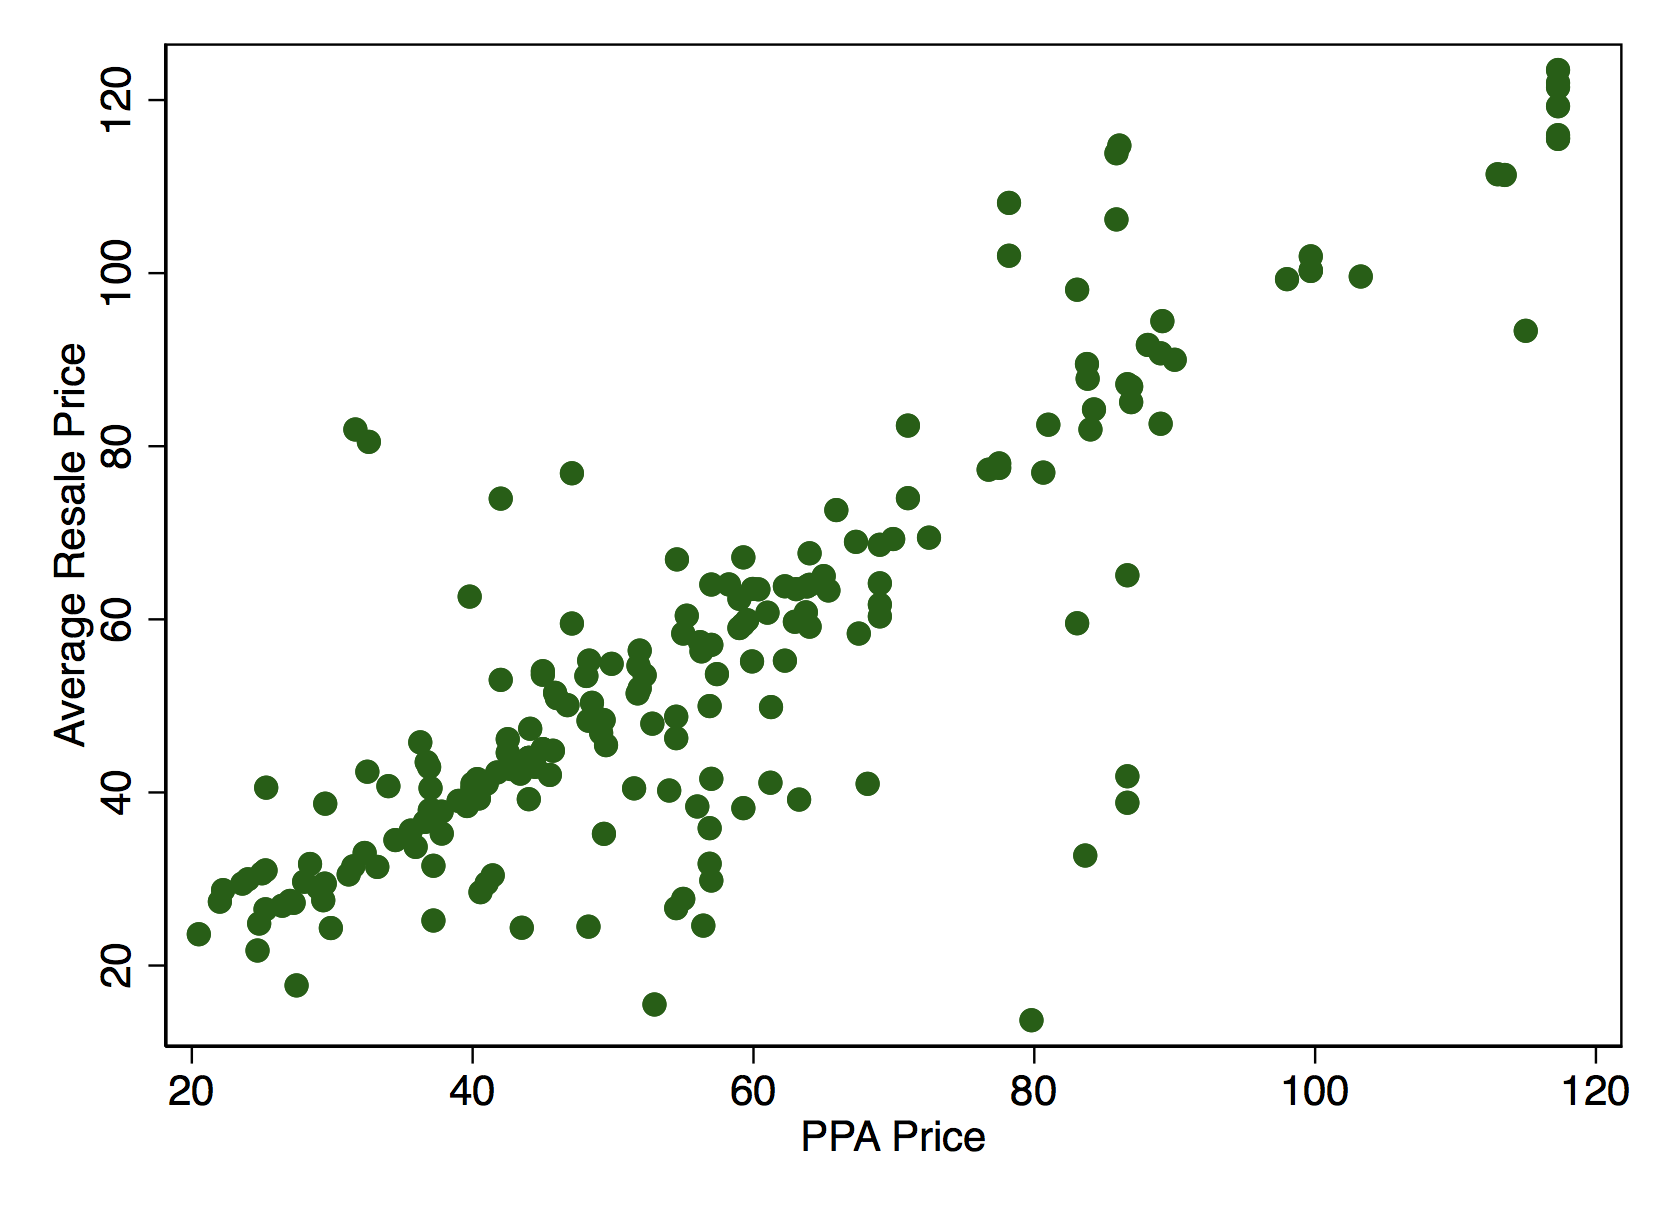
\includegraphics[width=0.75\textwidth]{../output/figures/resale_vs_ppa_price.png}
\end{figure}

\paragraph*{Renewable Energy Certificates Data}

As of 2017, 29 states and Washington D.C. had enacted RPSs. Wind farms generate certificates for each unit of production, which they then sell to covered non-renewable generators. Unfortunately, these payments are not observed in the EIA data.

We construct estimates of the RPS payments available to wind farms in a given state-month using bid-ask data on RECs trades from all active state RECs markets dating to 2007 from Marex Spectron in May 2015. To account for the fact that some states allow covered non-renewable entities to obtain credits from qualifying renewable facilities outside the state, we combine these state level prices with annual estimates of cross-state REC compliance flows from Lawrence Berkeley National Lab.\footnote{More information on this project tracking cross-state RECs at \href{https://emp.lbl.gov/projects/renewables-portfolio}{https://emp.lbl.gov/projects/renewables-portfolio}.} This expected REC payment is added to the average resale price to get marginal revenue each period. 





\clearpage
\section{Negative Price Analysis Details \label{Appendix:NegativePrices}}
\setcounter{figure}{0}  \renewcommand{\thefigure}{C.\arabic{figure}} 
\setcounter{table}{0}  \renewcommand{\thetable}{C.\arabic{table}} 

This appendix provides more detail on the data on negative prices and emissions rates used in Section~\ref{sec:Mechanism}. We collect high-frequency price data at multiple locations from six large U.S. electricity markets: California (CAISO), Texas (ERCOT), the Eastern U.S. (PJM), the Midwest (MISO), New England (ISONE), and New York (NYISO). Table~\ref{tab:Frequency-of-Negative} summarizes the likelihood of negatives prices in these six markets. The first panel contains summary statistics for all nodes (i.e., locations), and the second panel contains summary statistics for the set of nodes that are closest to each wind farm in our sample. Within the set of nodes near wind farms, negative prices are more common in California, Texas, and the Midwest. They are also less common in the summer, when demand is higher, and have generally been coming down over this sample period. Comparing across the two panels, negative prices are more common at nodes near wind farms than across all nodes in each ISO, although the difference varies considerably.

\begin{table}[h]
    \begin{centering}
    \caption{Frequency of Negative Prices in Six ISOs (2011-2014)\label{tab:Frequency-of-Negative}}
    \par\end{centering}
    \vspace{-15pt}
    
    \begin{center}
\begin{tabular}{lcccccc}
\hline \noalign{\smallskip} & CAISO & ERCOT & ISONE & MISO & NYISO & PJM\\
\noalign{\smallskip}\hline \textbf{\underline{All nodes}} &  &  &  &  &  & \\
Mean & 3.88 & 1.41 & 0.08 & 3.39 & 0.65 & 0.55\\
Median & 2.53 & 0.00 & 0.00 & 1.25 & 0.40 & 0.13\\
95th pctile & 16.26 & 8.21 & 0.00 & 14.43 & 2.02 & 2.42\\
\noalign{\smallskip}Summer(mean) & 4.59 & 0.74 & 0.01 & 2.95 & 0.67 & 0.69\\
Post 2012 (mean) & 2.24 & 0.59 & 0.16 & 3.18 & 0.74 & 0.40\\
\textbf{\underline{Near wind}} &  &  &  &  &  & \\
\noalign{\smallskip}Mean & 4.07 & 4.73 & 0.09 & 6.12 & 1.20 & 0.99\\
Summer(mean) & 2.25 & 0.31 & 0.01 & 3.72 & 0.83 & 0.82\\
Post 2012 (mean) & 2.52 & 1.30 & 0.18 & 6.21 & 1.66 & 0.84\\
\textbf{\underline{CO2 MOER}} &  &  &  &  &  & \\
\noalign{\smallskip}Mean & 896 & 1,378 & 1,262 & 1,870 & 1,312 & 1,776\\
Mean(weighted) & 873 & 1,457 & 1,169 & 1,916 & 1,408 & 1,778\\
Correlation & -0.46 & 0.60 & -0.72 & 0.69 & 0.41 & 0.02\\
\noalign{\smallskip}\hline\end{tabular}\\
\end{center}

    
    \footnotesize
    
    Frequencies (in percentage points) based on hourly nodal price data from the six listed ISOs, collapsed to the node-month level. Summer months are defined by the NOx regulation season, when begins in May and ends in October. In the second Section, the sample is restricted to nodes that are the closest node to a wind farm in the sample. The third Section of the table presents the average marginal operating emissions rate in pounds of carbon dioxide per MWh estimated for each ISO by \citet{callaway_location_2018}. The second row re-weights the average by the share of negative prices in each ISO-season-hour. The final row presents the correlation between negative prices and marginal operating emissions rates across 48 season-hour averages for each ISO.
\end{table}

We augment the negative price data with marginal operating emissions rates from \citet{callaway_location_2018}. \citet{callaway_location_2018} provide estimates of the average marginal operating emissions rate of generating resources by hour of day and season for each ISO, which we replicate in the first panel of Figure~\ref{fig:moer_np_season}. The second panel contains the frequency of negative prices for the same hours and seasons. Electricity prices typically fall below zero when demand is lowest, during the middle of the night. However, for four of the six ISOs, marginal emissions are actually \emph{higher} at night than during peak hours. This is not surprising due to the fact that natural gas is likely to be on the margin during the day, whereas coal is more likely to be on the margin at night. Comparing across the seasons, average emission rates are fairly constant, compared to the variation in negative price frequency.

%\subsection{Marginal Operating Emissions Rates from \citet{callaway_location_2018}}

\clearpage
\begin{figure}[H]
\noindent\begin{minipage}[t]{1\textwidth}%
\begin{center}
\caption{Marginal Emissions and Negative Price Frequency by Hour of Day and Season \label{fig:moer_np_season}}
\par\end{center}
\begin{center}
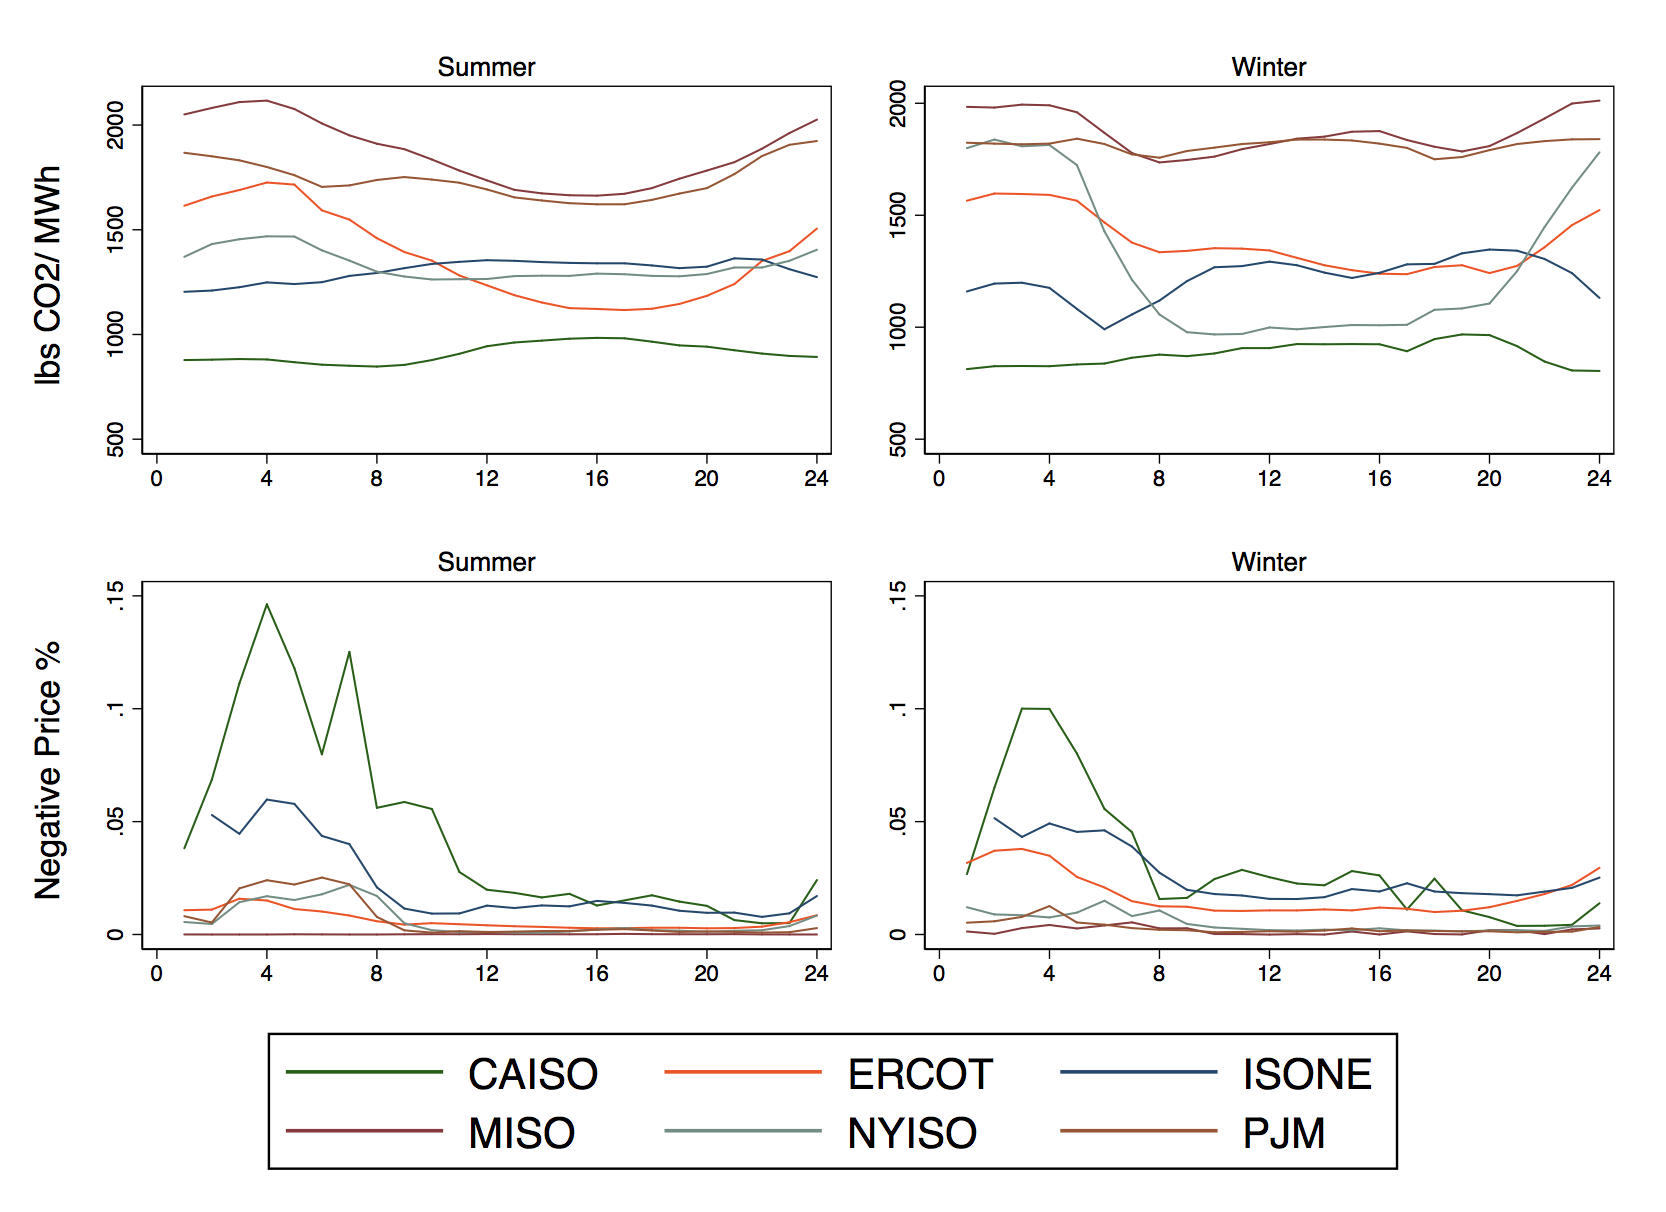
\includegraphics[width=1\textwidth]{../output/figures/moer_np_season.png}
\par\end{center}
Estimates of marginal operating emissions rates by hour of day and season were extracted from the appendix of \citet{callaway_location_2018}. Figures in the second row plot the mean share of negative price hours by ISO for the same hours and seasons. %
\end{minipage}
\end{figure}

The third panel of Table~\ref{tab:Frequency-of-Negative} contains average marginal emissions rates for each ISO. These emissions rates vary across regions, but are still positive and large everywhere, even when weighted by the negative prices in each ISO-season-hour. Finally, we present the correlation between negative prices and marginal operating emissions rates in the last row of Table~\ref{tab:Frequency-of-Negative}. In four of the six electricity markets, negative prices are positively correlated with marginal operating emissions rates, suggesting that the \textit{external} social value of wind energy during these hours is at least as high as during other time periods.




\clearpage
\section{Additional Tables and Figures}
\setcounter{figure}{0}  \renewcommand{\thefigure}{D.\arabic{figure}} 
\setcounter{table}{0}  \renewcommand{\thetable}{D.\arabic{table}} 

%\subsection{Linear RD Results \label{sec:LinearRD}}

\begin{table}[H]
\caption{IV Results Sensitivity: Linear RD \label{tab:rdd_cf_linear}}
\begin{center}{\footnotesize{}{
\def\sym#1{\ifmmode^{#1}\else\(^{#1}\)\fi}
\begin{tabular}{l*{6}{c}}
\toprule
                &\multicolumn{1}{c}{(1)}         &\multicolumn{1}{c}{(2)}         &\multicolumn{1}{c}{(3)}         &\multicolumn{1}{c}{(4)}         &\multicolumn{1}{c}{(5)}         &\multicolumn{1}{c}{(6)}         \\
\midrule
1603 Grant      &   -3.697\sym{***}&   -2.893\sym{**} &   -3.156\sym{***}&   -6.376\sym{**} &   -4.774\sym{**} &   -1.346         \\
                &  (1.351)         &  (1.238)         &  (1.170)         &  (2.520)         &  (2.241)         &  (2.244)         \\
\addlinespace
Regulated       &                  &   -1.371         &   -5.446\sym{***}&                  &   -2.305         &   -5.980\sym{***}\\
                &                  &  (1.685)         &  (1.970)         &                  &  (1.881)         &  (1.943)         \\
\addlinespace
PPA             &                  &   -0.600         &   -2.618\sym{***}&                  &   -0.465         &   -2.704\sym{***}\\
                &                  &  (1.056)         &  (0.925)         &                  &  (1.063)         &  (0.952)         \\
\addlinespace
IPP             &                  &   -1.408         &   -2.514\sym{*}  &                  &   -1.883         &   -3.105\sym{**} \\
                &                  &  (1.305)         &  (1.307)         &                  &  (1.337)         &  (1.364)         \\
\addlinespace
Potential Capacity Factor&                  &    0.503\sym{***}&    0.553\sym{***}&                  &    0.503\sym{***}&    0.560\sym{***}\\
                &                  & (0.0368)         & (0.0386)         &                  & (0.0383)         & (0.0362)         \\
\addlinespace
Var(Wind Speed) &                  &   0.0637         &   -0.432\sym{***}&                  &  0.00692         &   -0.433\sym{***}\\
                &                  &  (0.155)         &  (0.107)         &                  &  (0.160)         &  (0.108)         \\
\addlinespace
log(Capacity)   &                  &   -0.605         &    0.580         &                  &   -0.643         &    0.600         \\
                &                  &  (0.430)         &  (0.470)         &                  &  (0.423)         &  (0.478)         \\
\midrule
Regression Type &     2SLS         &     2SLS         &     2SLS         &     2SLS         &     2SLS         &     2SLS         \\
Controls        &        N         &        Y         &        Y         &        N         &        Y         &        Y         \\
State FE        &        N         &        N         &        Y         &        N         &        N         &        Y         \\
Piecewise Trend &        N         &        N         &        N         &        Y         &        Y         &        Y         \\
N               &     8752         &     8752         &     8752         &     8752         &     8752         &     8752         \\
First-stage F-stat.&      148         &      169         &      113         &       38         &       32         &       22         \\
\bottomrule
\end{tabular}
}
}\end{center}
\footnotesize
Data include a balanced panel of monthly observations from 2010 to 2014 for all wind farms. The first three columns replicate the IV results in Table~\ref{tab:rdd_cf}. For columns 4 - 6, distance to the policy cutoff, and that distance interacted with the a post-policy indicator are included as controls. All models contain year-month dummies. Standard errors clustered by wind farm reported in parentheses.
\end{table}


\begin{table}[h]
\begin{centering}
\caption{Matching Results Sensitivity: Matching on Potential Capacity Factor \label{tab:matching_group_ptnlcf}}
{
\def\sym#1{\ifmmode^{#1}\else\(^{#1}\)\fi}
\begin{tabular}{l*{5}{c}}
\toprule
                    &\multicolumn{1}{c}{(1)}         &\multicolumn{1}{c}{(2)}         &\multicolumn{1}{c}{(3)}         &\multicolumn{1}{c}{(4)}         &\multicolumn{1}{c}{(5)}         \\
\midrule
1603 Grant          &      -2.942\sym{***}&      -3.884\sym{***}&      -3.120\sym{***}&      -2.712\sym{**} &      -2.780\sym{**} \\
                    &     (0.719)         &     (1.027)         &     (1.067)         &     (1.098)         &     (1.196)         \\
\midrule
Sample              &         All         &     Matched         &     Matched         &     Matched         &     Matched         \\
FEs                 &       State         &       State         &       Group         &     Group*Y         &   Group*Y*M         \\
R-sq.               &       0.615         &       0.633         &       0.655         &       0.669         &       0.789         \\
N                   &       21303         &       12885         &       12885         &       12885         &       12885         \\
\bottomrule
\end{tabular}
}

\par\end{centering}
\footnotesize

The matched sample was constructed using coarsened exact matching on state, regulatory status, entity type, capacity, and potential capacity factor. All models include the controls listed in the IV models in Table~\ref{tab:rdd_cf}: log capacity, potential capacity factor, and wind speed variance, as well as dummies for whether the plant is regulated, whether it is an IPP, the presence of a PPA, and month of sample. All models also include cohort dummies. Standard errors, clustered at the plant level, are reported in parentheses.
\end{table}

\begin{table}[h]
\begin{centering}
\caption{Sensitivity of Matching Estimates to Geographic Restrictions, Matching on Potential Capacity Factor \label{tab:matching_table_cf_ptnlcf}}
{
\def\sym#1{\ifmmode^{#1}\else\(^{#1}\)\fi}
\begin{tabular}{l*{4}{c}}
\toprule
                    &\multicolumn{1}{c}{(1)}         &\multicolumn{1}{c}{(2)}         &\multicolumn{1}{c}{(3)}         &\multicolumn{1}{c}{(4)}         \\
\midrule
1603 Grant          &      -1.933\sym{**} &      -1.692\sym{**} &      -1.178         &      -2.712\sym{**} \\
                    &     (0.773)         &     (0.811)         &     (0.858)         &     (1.098)         \\
\midrule
\# Pre-PTC          &         137         &         115         &         115         &         120         \\
\# Post-PTC         &          50         &          49         &          43         &          32         \\
\# Post-1603        &         128         &          98         &          90         &          95         \\
Region              & Nerc-1(ISO)         &         ISO         &    Nerc*ISO         &       State         \\
R-sq.               &       0.674         &       0.694         &       0.690         &       0.669         \\
N                   &       15851         &       13195         &       12758         &       12885         \\
\bottomrule
\end{tabular}
}

\par\end{centering}
\footnotesize

Matched samples constructed using coarsened exact matching on geographies listed in the table, regulatory status, entity type, capacity, and potential capacity factor. All models include the controls listed in the IV models in Table~\ref{tab:rdd_cf}: log capacity, potential capacity factor, and wind speed variance, as well as dummies for whether the plant is regulated, whether it is an IPP, the presence of a PPA, and month of sample. All models also include cohort dummies, matched group-year fixed effects, and state fixed effects. Standard errors, clustered at the plant level, are reported in parentheses.
\end{table}


\clearpage

%\subsection{Wind Farm Locations by Period and Subsidy}

\begin{sidewaysfigure}[h] \centering
	\caption{New Wind Farms by Subsidy (2009-2012)\label{map:2009to2012}}
	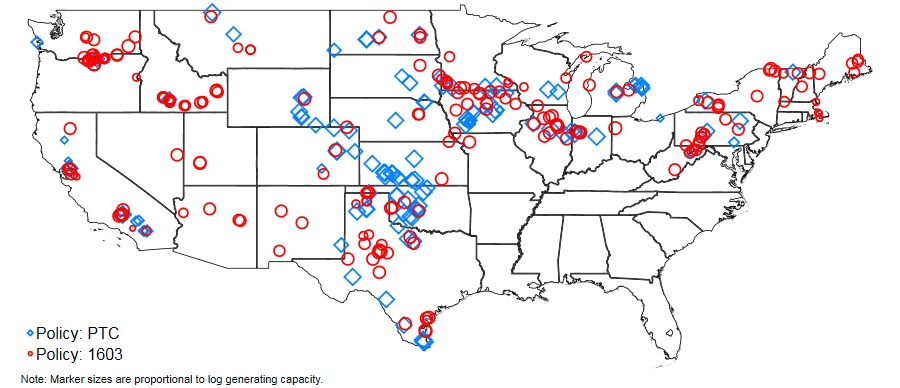
\includegraphics[width=\textwidth]{../output/figures/map_2009to2012.png}
\end{sidewaysfigure}

\begin{sidewaysfigure}[h] \centering
	\caption{New Wind Farms by Subsidy (2008-2009)\label{map:2008to2009}}
	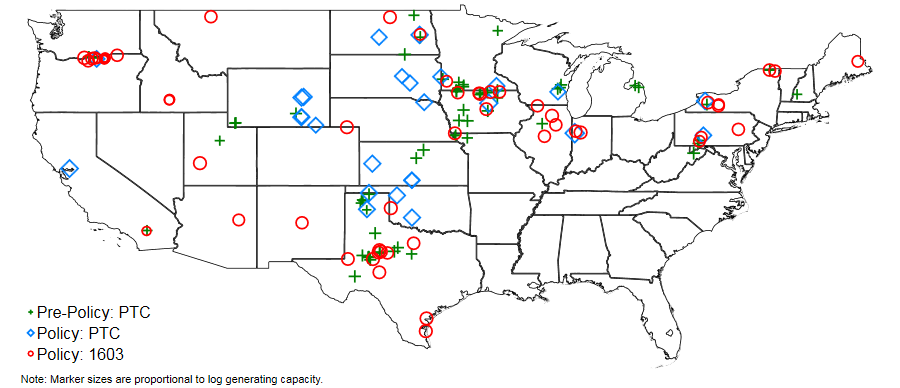
\includegraphics[width=\textwidth]{../output/figures/map_2008to2009.png}
\end{sidewaysfigure}

%\subsection{Additional Data on Power Plant Proposal and Completion}

\begin{figure}[h] \centering
\caption{Share of Plants Ever Completed, Plotted by Year of Initial Expected Completion\label{fig:proposed_ever_completed}}
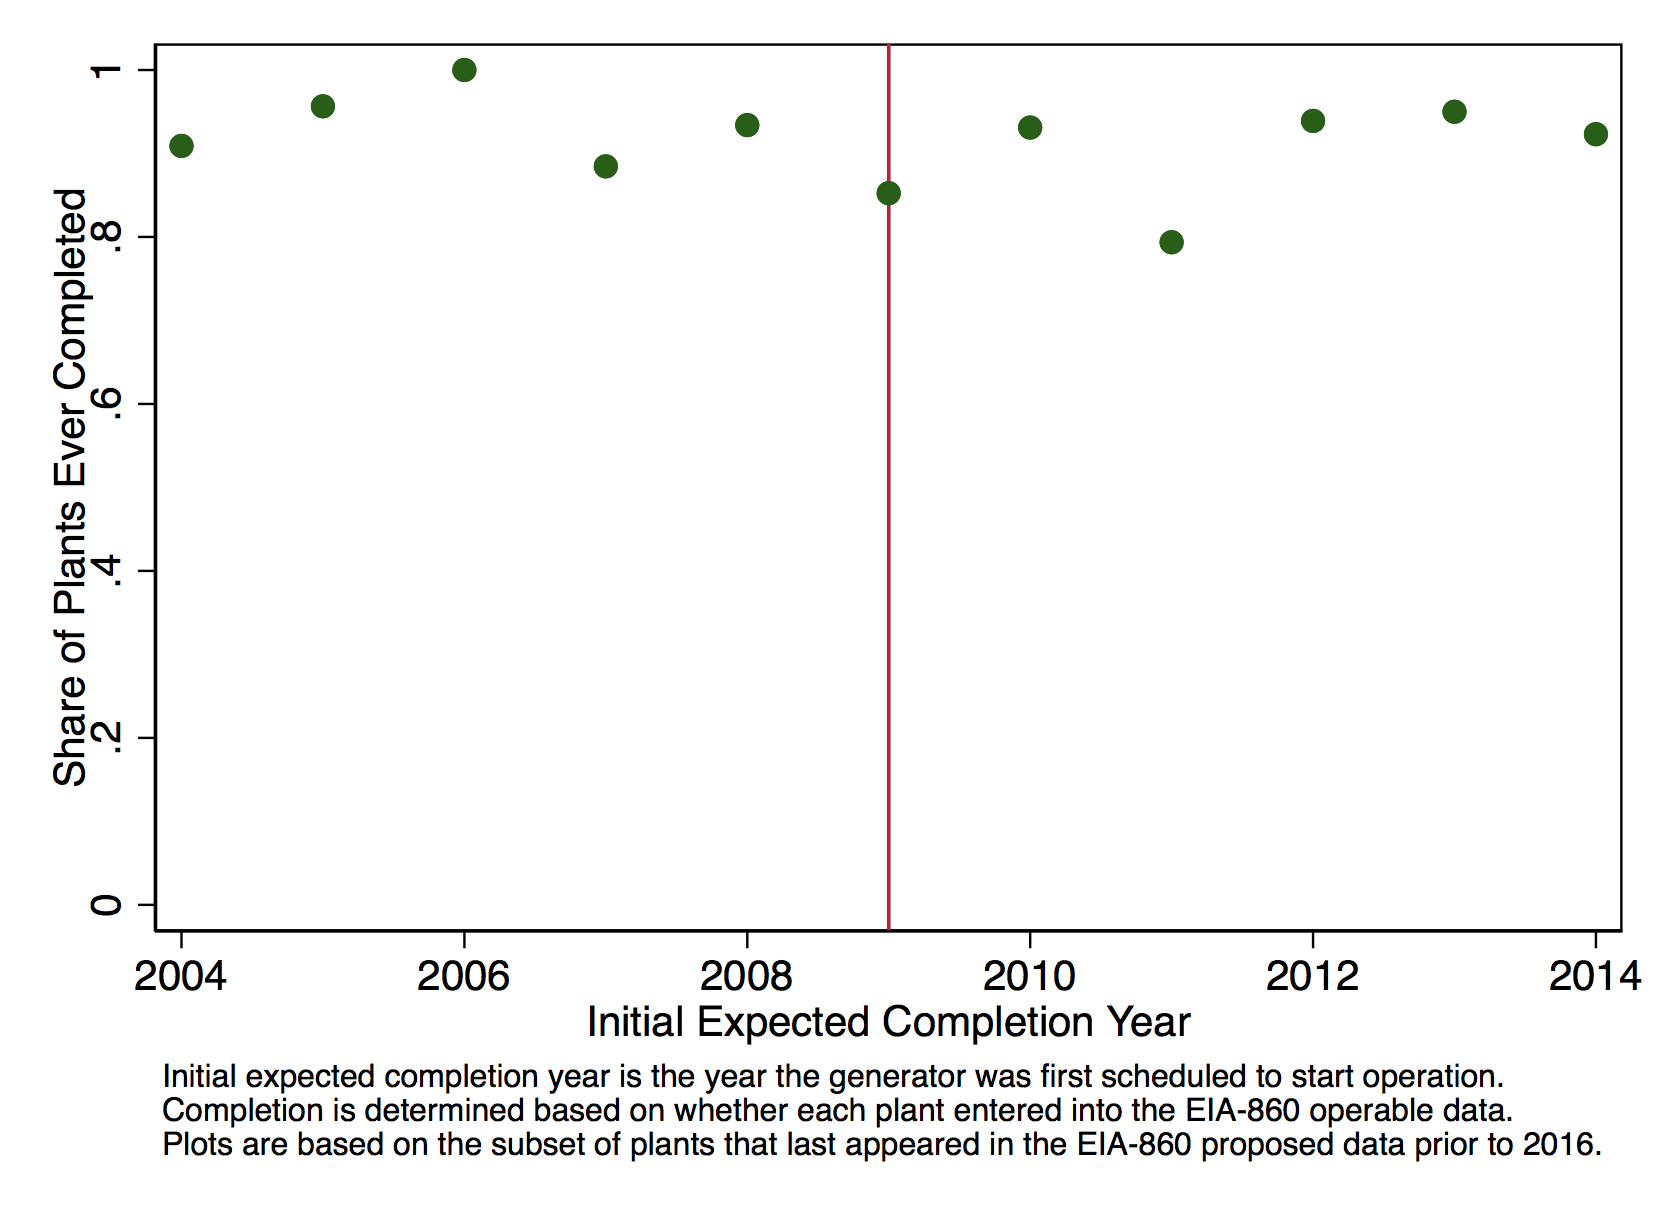
\includegraphics[width=0.75\linewidth]{../output/figures/proposal_data_ever_completed.png}
\end{figure}

\end{document}